\vspace{-0.2cm}
\begin{flushright}
\emph{``For the things we have to learn before we can do them, we learn by doing them.''}\\
Aristotle, in \textit{The Nicomachean Ethics}, IV$^\text{th}$ century BC
\end{flushright}
\vspace{0.4cm}

Uncertainties about the future along with a large variety of \gls{IAMs} yield an even larger variety of \gls{GHG} emissions reduction pathways \cite{nicolas2021robust}. For instance, several studies \cite{IPCC_CO2_budget,steffen2018trajectories} advocate for actions to take in the near future, especially to keep on track within the 1.5°C (if not, 2°C) increase of global temperature above pre-industrial levels by the end of the century. On the contrary, using his top-down model DICE, \citet{nordhaus2014question} states that immediate and drastic actions are not compulsory to meet the ambition of climate change mitigation. 

To navigate through the myopic transitions not constrained by a prescribed \ce{CO2}-trajectory and investigate the efficiency of different policies, we apply the reinforcement learning approach detailed in Section \ref{sec:meth:RL} on the case study of Belgium. Besides the environment, \ie the myopic transition pathway of the whole-energy system via EnergyScope Pathway (see Chapter \ref{chap:chap_methodo}), the first part of this chapter presents the three key features of interaction between the agent, optimizing its policy, and the environment: actions, states and reward.  Then, the results of this policy optimisation point out strategies to follow, \ie \textit{sweet spots}, in the transitions under uncertainties as well as \textit{no-go zones} where the chances of succeeding the transition, \ie respecting the \ce{CO2}-budget, are very limited. Finally, these results are compared with references, \ie the perfect foresight and the myopic optimisation of the transition under the same uncertainties but without the trained \gls{RL}-agent that can support this transition thanks to its learned policy.

\section*{Contributions}
\label{sec:RL:contributions}
Applying the \gls{RL} approach to the optimization of the myopic transition pathway of a whole-energy system presents several novelties. First of all, as introduced in Section \ref{subsec:meth_RL_fundamentals}, when applied to energy systems, \gls{RL} is more dedicated either to smaller scale systems (\eg \gls{BEMS}, vehicles and energy devices) or to sector-specific, often the power sector, problems (\eg dispatch problems, energy markets and grid) \cite{perera2021applications}. In our case, the sector-coupling, the long-term goal at the end of a multiple-steps transition and the number of uncertain parameters make this application new for \gls{RL}.

Applying \gls{RL} to the optimisation environment of EnergyScope Pathway myopic,  rather than a simulation environment, allows building a hierarchical multi-objective optimisation framework: while the objective of the environment remains the minimisation of the total ``transition'' cost (on the concerned limited time window), the agent optimises its strategy to respect the \ce{CO2}-budget. 

Comparing the \gls{RL}-based results with more conventional approaches, \ie perfect foresight optimisation, highlights the added-value brought by this approach in the exploration of myopic transition pathways.

Usually, applications of \gls{RL} focus more on the result of the learning process, the optimised policy, for optimising the control of a system \cite{perera2021applications}. This thesis also investigates the learning episodes themselves to explore the field of possibilities to succeed the transition.


\section{Definition of the actions, reward and states}
\label{sec:RL:act_states_rew}
As already introduced in Section \ref{subsec:meth_RL_algo}, the environment with which the \gls{RL}-agent interacts is the optimisation of the transition pathway of a whole-energy system on a specific time window, \eg 2020-2030 then 2025-2035 and so on, until 2040-2050 (see Figure \ref{fig:Schematics_RL}). In a nutshell, starting from the initial state of the environment (\ie the whole-energy system in 2020), the agent takes a set of actions that influence the environment, \ie that affects parameters of the Linear Programming in EnergyScope Pathway. Then, the window 2020-2030 is optimised via EnergyScope. Some of the outputs of this optimisation feed the agent with either the new state of the system or the reward, \ie telling the agent how good the actions were at the state the agent took it. Based on the new state and the reward, the agent takes another set of actions and the window 2025-2035 is optimised. This goes on until 2050.



\subsection{Actions}
\label{subsec:RL:act_states_rew:act}

Defining the levers of action, the core of the policy, to support the transition of a country-size whole-energy system is challenging, especially when accounting for political and socio-technical aspects \cite{castrejon2020making}. In our work, focusing only on the techno-economic aspect, we assume that the actions taken by the agent are directly implemented and impacting the environment. In other words, considering only the techno-economic lens, there is no moderation nor contest towards the agent's actions, as the objective is to assess how far and when within the transition to push the different levers of action. Given the overall objective of the agent to succeed the transition, \ie respecting the \ce{CO2}-budget by 2050, we have defined the actions in this sense. The first action, $\mathrm{act}_{\mathrm{gwp}} \in [0,1]$, aims at limiting the emissions at the representative year ending the concerned time window, $\textbf{GWP\textsubscript{tot}}(y_{\text{end of the window}})$, between the level of emissions in 2020, \ie $\textbf{GWP\textsubscript{tot}}(2020)=123\,\text{Mt}_{\ce{CO2},\text{eq}}$, and carbon-neutrality:

\begingroup
\belowdisplayskip=2pt
\abovedisplayskip=2pt
\begin{flalign} 
\label{eq:RL:act_gwp}
&\textbf{GWP\textsubscript{tot}}(y_{\text{end of the window}})\leq \mathrm{act}_{\mathrm{gwp}} \cdot \textbf{GWP\textsubscript{tot}}(2020). &
\end{flalign}
\endgroup

\noindent
This action is equivalent to setting a national \ce{CO2}-quota.

Three additional actions support the strict limitation of yearly emissions: limiting the consumption of oil, fossil gas and coal. Out of the total \gls{GHG} emissions in Belgium in 2020, oil (\ie so-called ``\gls{LFO}'' in the model) and fossil gas account for roughly 40\% and 31\%, respectively. In 2020, solid fossil fuels (\ie so-called ``coal'' in the model) is much less consumed than oil and gas: \ie 28\,TWh of solid fossil fuels versus 159 and 142\,TWh for oil and fossil gas, respectively. Even though its cost (17€/MWh) makes coal cost-competitive, it is a highly-emitting resource, 0.40\,kt$_{\ce{CO2},\text{eq}}$/GWh. For these reasons, three independent actions limit the consumption of these three fossil resources up to the level of consumption in 2020, $\textbf{Cons\textsubscript{fossil gas}}(2020)$, $\textbf{Cons\textsubscript{LFO}}(2020)$ and $\textbf{Cons\textsubscript{coal}}(2020)$,  over the entire concerned time window, except the first one as this year is the initial condition of the time window and cannot be optimised any more:

\begingroup
\belowdisplayskip=2pt
\abovedisplayskip=2pt
\begin{flalign} 
\label{eq:RL:act_NG}
&\textbf{Cons\textsubscript{fossil gas}}(y)\leq \mathrm{act}\textsubscript{fossil gas} \cdot \textbf{Cons\textsubscript{fossil gas}}(2020) & \forall y \in \text{time window}\\
\label{eq:RL:act_LFO}
&\textbf{Cons\textsubscript{LFO}}(y)\leq \mathrm{act}\textsubscript{LFO} \cdot \textbf{Cons\textsubscript{LFO}}(2020) & \forall y \in \text{time window}\\
\label{eq:RL:act_COAL}
&\textbf{Cons\textsubscript{coal}}(y)\leq \mathrm{act}\textsubscript{coal} \cdot \textbf{Cons\textsubscript{coal}}(2020) & \forall y \in \text{time window}
\end{flalign}
\endgroup

\noindent
where $\mathrm{act}\textsubscript{fossil gas}$, $\mathrm{act}\textsubscript{LFO}$ and $\mathrm{act}\textsubscript{coal}$ can take values between 0 and 1. These complete the action space of the agent, $A\in \mathbb{R}^4_{[0,1]}$ (see Figure \ref{fig:Schematic_actions}).

\begin{figure}[!htbp]
\centering
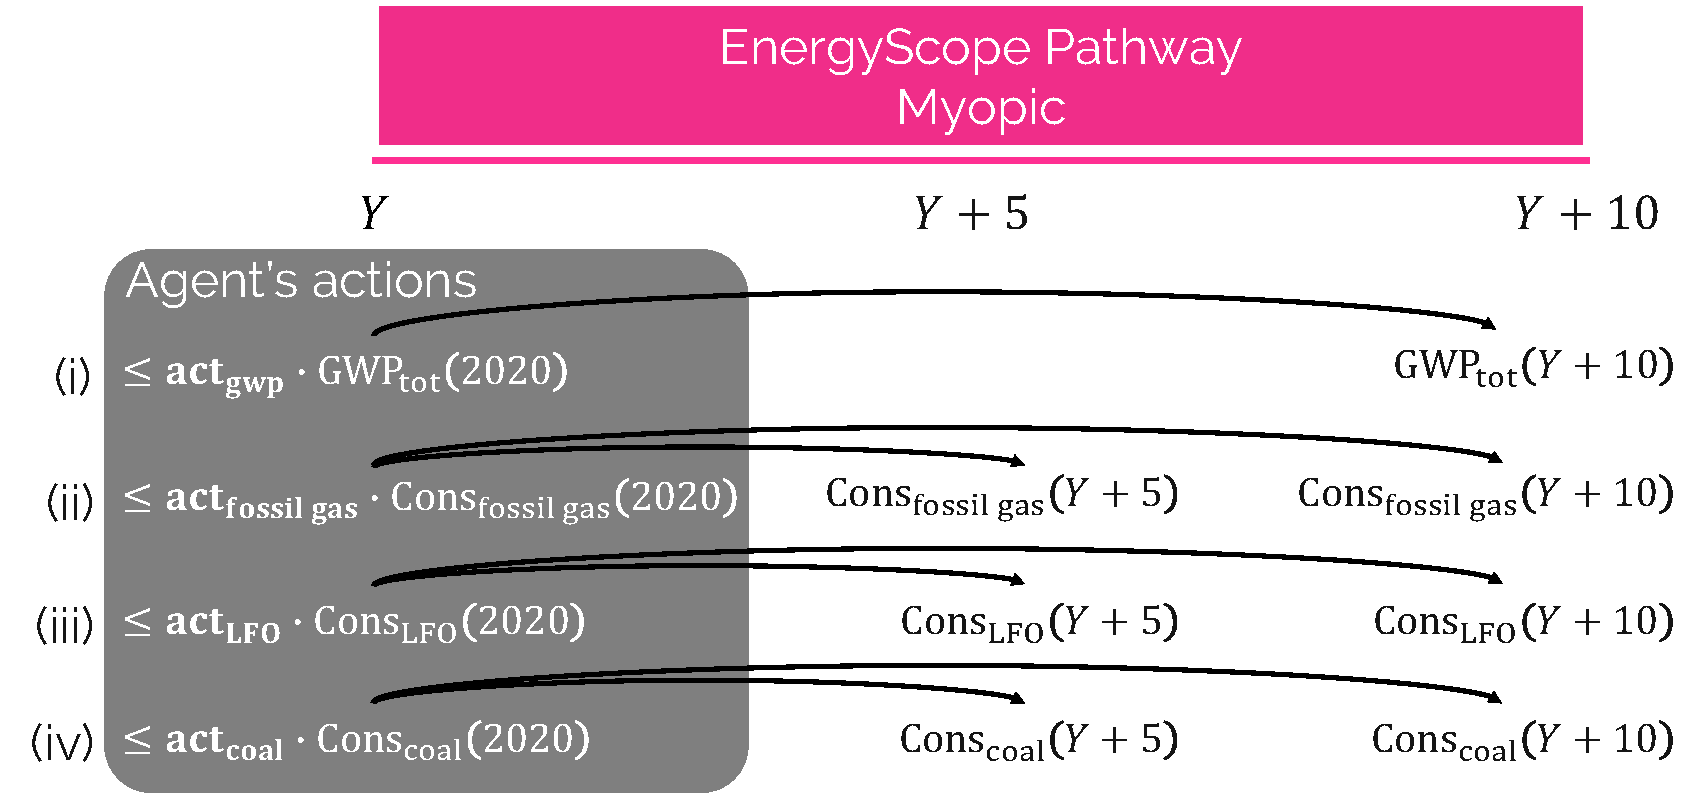
\includegraphics[width=0.8\textwidth]{Schematic_actions.pdf}
\caption{Actions available to the decision-maker. Taken at the beginning of the time-window to optimise (year $Y$), the four actions impact (i) the emissions of the system at the end of the time-window (year $Y+10$) and, (ii-iv) the consumption of fossil gas, LFO and coal at years $Y+5$ and $Y+10$. Unlike the first action that sets a target for the end of the time-window, the last three aim at limiting the consumption of these fossil resources over the whole time-window.}
\label{fig:Schematic_actions}
\end{figure} 

\subsection{Reward}
\label{subsec:RL:act_states_rew:rew}

When the reward is not properly defined, the agent may optimise its policy for an unintended objective, leading to undesired or subotpimal behavior, \ie the so-called misalignment of the learning objective \cite{christiano2017deep}. Even worse, it can lead to reward hacking (or reward tampering) where the agent exploits loopholes in the reward function to achieve higher rewards without actually performing the desired task \cite{amodei2016concrete}. On the contrary, a proper definition of the reward function increases the sample efficiency, \ie requiring less episode to converge to the optimal policy.  It also makes the policy more stable and able to withstand variations and uncertainties in the environment \cite{henderson2018deep}.

Through its maximisation of the expected return (see Section \ref{subsec:meth_RL_algo}), a \gls{RL}-agent is as sensitive to positive reward, \ie the carrot, as negative reward, \ie the stick.  When the former encourages desired behaviours, the latter can be seen as a penalty or a punishment and discourages the undesirable behaviours \cite{sutton2018reinforcement}. In our case, we have decided to combine these two approaches (see Figure \ref{fig:Reward}).

\begin{figure}[!htbp]
\centering
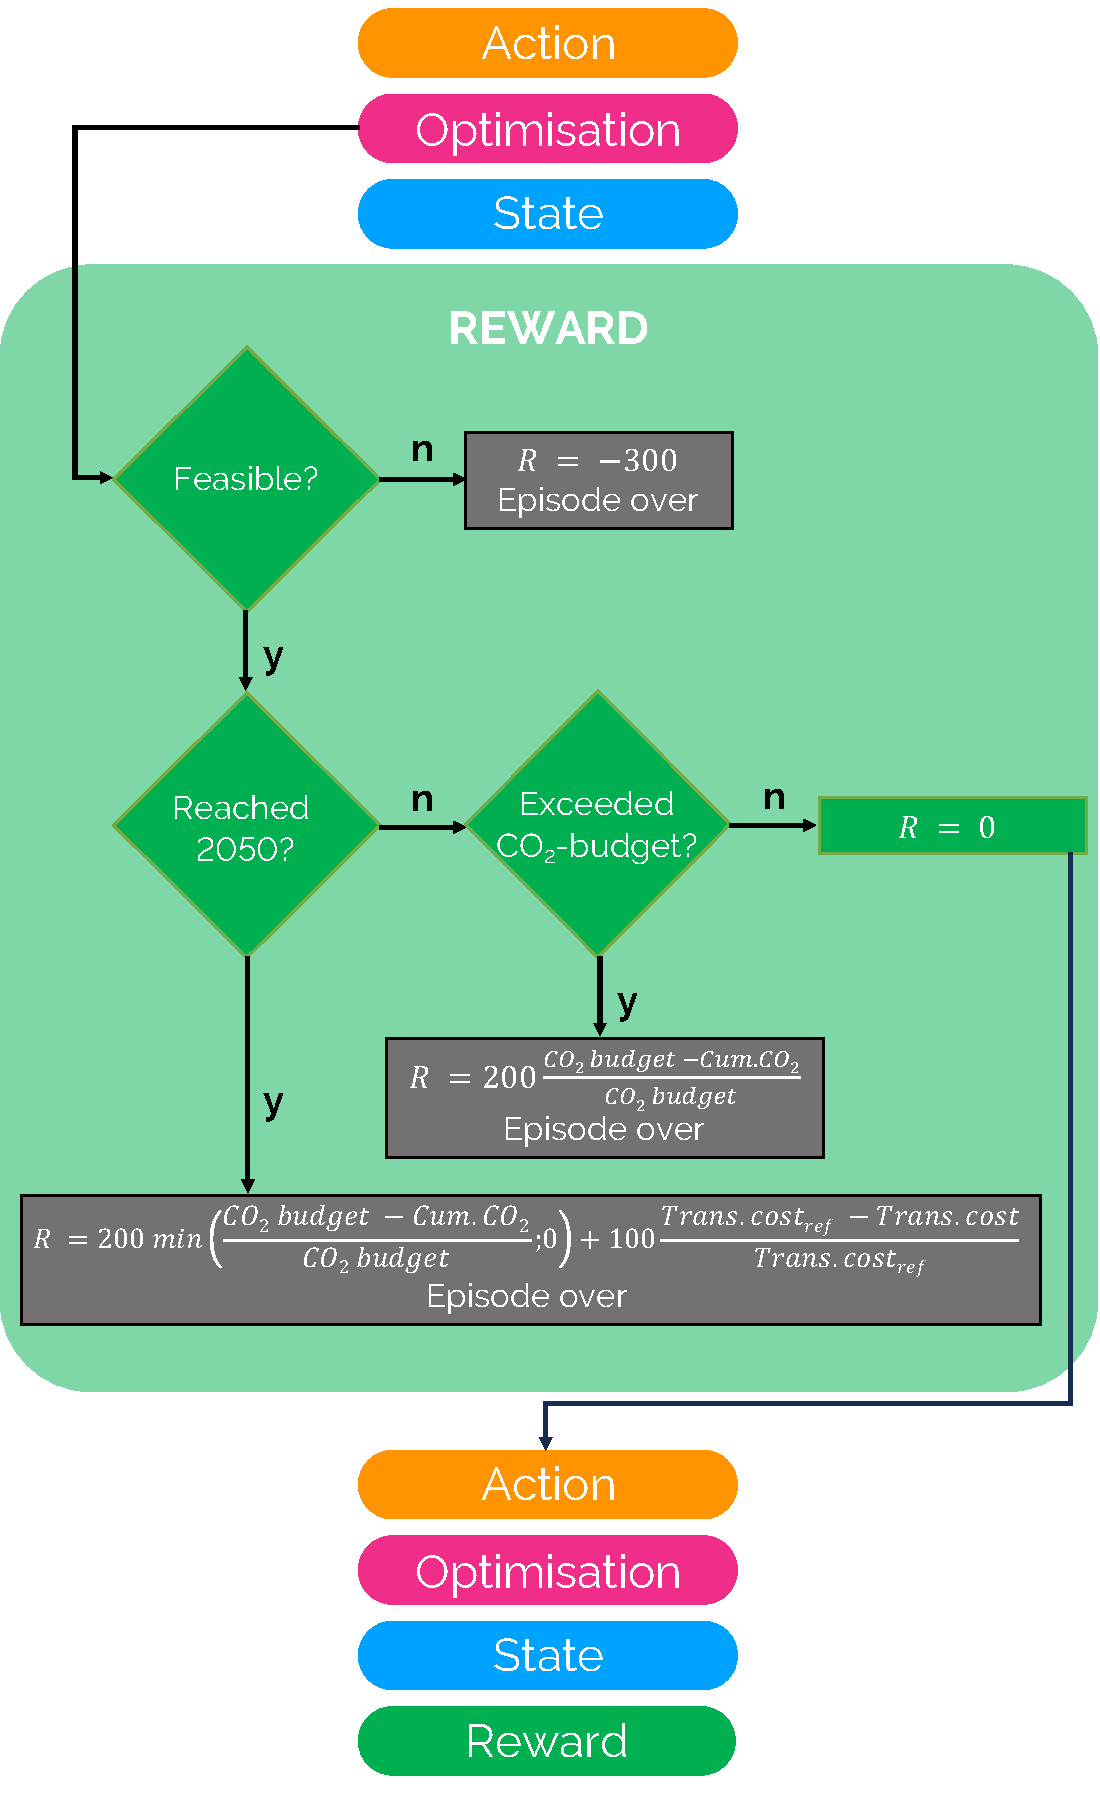
\includegraphics[width=0.8\textwidth]{Reward.pdf}
\caption{Reward function, $R$. Before reaching 2050, the episode is prematurely ended and a negative reward is given if the optimisation is infeasible or if the \ce{CO2}-budget is exceeded. If the optimisation provides a solution and the \ce{CO2}-budget is not exceeded, the episode continues. Finally, if the episode goes until 2050, the reward is a weighted sum between the capped cumulative emissions and the total transition cost, and the episode terminates. After terminating an episode, the process starts over at the initial state, \ie 2020.}
\label{fig:Reward}
\end{figure} 

The reward function is defined in three steps. First of all, taking a set of actions at a certain state might lead to an infeasible optimisation problem. In other words, as actions have a direct impact on some constraints of the problem, they might limit too much the feasible domain to the point where no solution can be found. For instance, the extreme case of aiming at carbon-neutrality, \ie $\mathrm{act}_{\mathrm{gwp}}=0$, and forbidding the use of the three aforementioned fossil fuels, \ie $\mathrm{act}\textsubscript{fossil gas}=\mathrm{act}\textsubscript{LFO}=\mathrm{act}\textsubscript{coal}=0$,  from the beginning of the transition makes the optimisation impossible to solve. In this case, the episode is prematurely ended and the reward is ``highly'' negative, -300. If the optimisation is feasible and the end of the transition, \ie 2050, is not reached, the cumulative emissions so far are evaluated. On the one hand, if these cumulative emissions exceed the \ce{CO2}-budget, $1.2\,\text{Gt}_{\ce{CO2},\text{eq}}$ (see Section \ref{sec:cs:CO2-budget}), the episode is also ended and a penalisation is given to the agent. This penalisation is proportional to the difference between the \ce{CO2}-budget and the actual cumulative emissions.  On the other hand, the episode continues with a zero reward if the \ce{CO2}-budget is not exceeded. Eventually, when reaching 2050, given the main objective of the agent to respect the \ce{CO2}-budget and not to be more ``\ce{CO2}-ambitious'', we cut short the contribution of the cumulative emissions as soon as they are lower or equal to the \ce{CO2}-budget.  On top of that, the reward function includes a secondary objective: the cumulative transition cost. To make the agent sensitive to the cost-impact of its policy, we added the total transition cost in the reward function where the \emph{Trans. cost$_{\text{ref}}$} on Figure \ref{fig:Reward} is equal to $1.1\cdot10^3$\,b€. This value comes from the mean of the total transition costs obtained through the \gls{GSA} performed on the perfect foresight transition pathway optimisation (see Section \ref{subsec:atom_mol:results_uq_cost}). In this final form of the reward, one will notice that overshooting cumulative emissions are more penalising than an overshooting transition cost, \ie weight of 200 for the emissions versus 100 for the cost. The values of these weights are the results of a trial and error to fine-tune the balance between more expensive successes and cheaper failures. This way, we observed that the agent first targeted the respect of the \ce{CO2}-budget and then, to a lesser scale, avoided reaching over-costly transitions.

\subsection{States}
\label{subsec:RL:act_states_rew:states}

Besides the reward, states are the other piece of information provided by the environment to the agent. In \gls{RL}, the purpose of states are to represent the current situation or configuration of the environment in which the agent operates. The primary function of states in RL is to provide the necessary context for the agent to choose appropriate actions based on its current observations and goals \cite{sutton2018reinforcement}. The challenge in the definition of the states is to provide enough information but not too much to avoid overwhelming the agent with non-informative features. 

Consequently, after testing several state spaces and observing the convergence of the reward, we have converged to a four-dimension state space characterizing the energy system at the end of the optimised time window. The first dimension is directly related to the main objective of the agent: respecting the \ce{CO2}-budget until 2050. Therefore, the cumulative emissions emitted so far up to the current step of the transition is the first dimension of the states. Similarly, the cumulative cost of the transition so far constitutes the second dimension of the states to inform the agent about the cost-impact of its actions on the environment. Finally, to enrich the level of details, we have added two other dimensions representative of the key-to-the-transition indicators identified in the Renewable Energy Directive (RED) III of the European Commission \cite{REDIII}: the share of renewables in the primary energy mix and, the energy efficiency. The former is computed as the share of local renewables (\ie wind, solar, hydro and biomass) and imported renewable energy carriers (\ie biofuels and electrofuels) in the total consumption of primary energy. Electricity imported from abroad is not considered in the set of renewable energy carriers even if it can be assumed to be fully renewable by 2050. Finally, even though energy efficiency is usually defined as the ratio between the \gls{FEC} and the primary energy mix, we decided to define this efficiency with a focus on the \gls{EUD}, like in the rest of this thesis. Where electricity, heat and non-energy \gls{EUD} are expressed in terms of energy content, we needed to convert passenger and freight transports into their respective \gls{FEC} to integrate them in the ratio. The information of efficiency fed back by the environment to the agent is the ratio between a ``hybrid'' \gls{EUD} and the consumption of primary energy resources.

\section{Convergence and learning process}
\label{sec:RL:learning}

Before comparing the agent's optimised policy with references, the first step consists in assessing the learning of the \gls{NN}, also called ``training''. For this, numerous episodes are played through the myopic optimisation of the transition pathway of Belgium. At the beginning of each episode, the agent starts with the Belgian energy system of 2020 (see Appendix \ref{app:bel_2020}). Then, a sample of values, drawn for the uncertain parameters, affects the model for the 2020-2030 time window. This single draw will affect the parameters for all the subsequent time windows (see Figure \ref{fig:ranges_transition}).  Then, the agent takes a set of actions, affecting the environment that feeds back the agent with a new state and a reward. This goes on until the end of the episode. For the next episode, similarly to the \gls{UQ} analysis (see Section \ref{sec:meth:UQ}), another sample of uncertain parameters is drawn following the quasi-random Sobol' sampling technique \cite{bratley2003implementing}.

We end this section with justifications of actions, reward and states implemented in this work as well as guidelines for researchers that would like to apply the RL approach on their own case study with their own model.

\subsection{Reward and success}
\label{subsec:RL:learning:rew_succ}

The learning phase has been split into batches of 500 steps,\ie 500 sequences of state-action-reward-new state. %For the first 100 steps of each batch, the \gls{RL}-model collects transitions before learning starts. This makes sure replay buffer is full enough for useful updates. 
At the end of each batch, the up-to-date policy, \ie the \gls{NN}, is saved. This way, we can assess the progress in the learning process and its convergence (see Figure \ref{fig:reward_success}).  The mean reward increases rapidly at the beginning of the learning process before reaching a plateau where the optimisation of the policy becomes more marginal.  As this successes drive indirectly the agent's optimisation, it shows that the reward function (see Figure \ref{fig:Reward}) leads towards more and more successes. However, given the wide range of uncertainty of some parameters and the agent's levers of action, this success rate stays limited at the end of the learning process. In other words, there are conditions where it is impossible for the agent to succeed the transition.

\begin{figure}[!htbp]
\centering
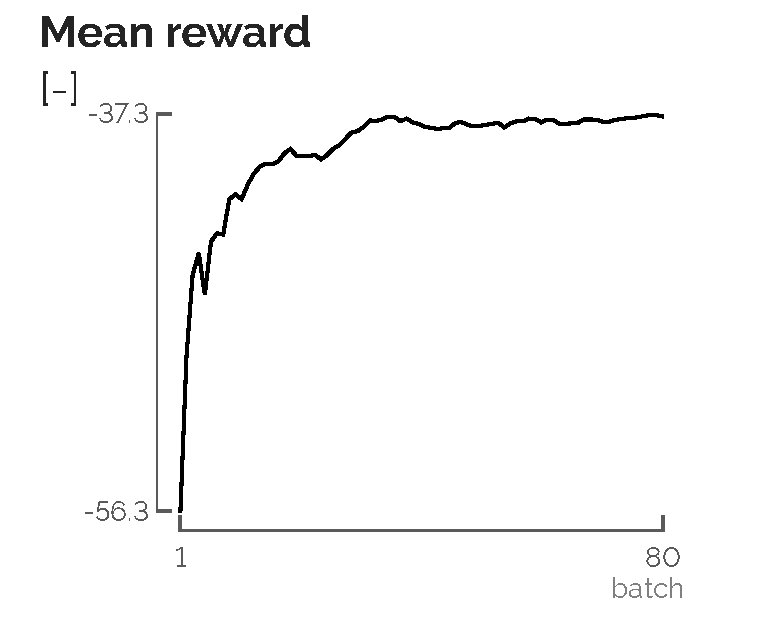
\includegraphics[width=0.49\textwidth]{Mean_reward.pdf}
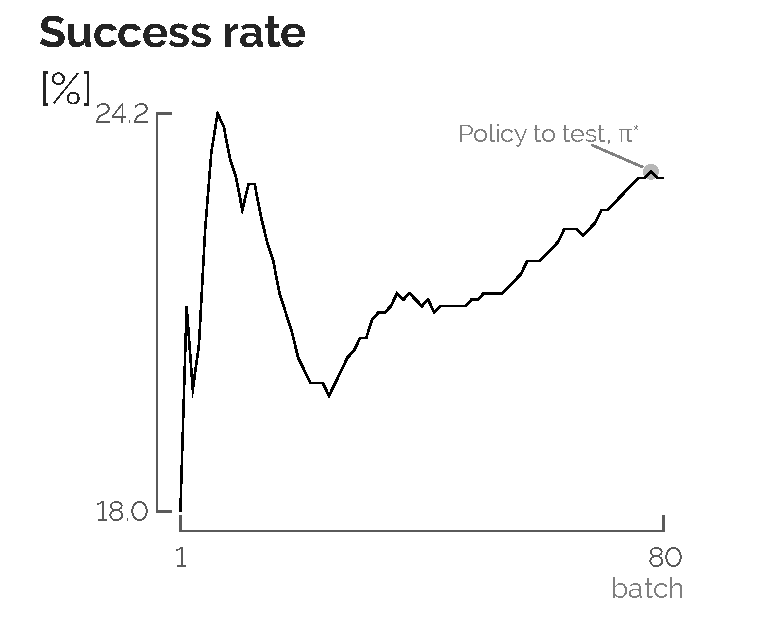
\includegraphics[width=0.49\textwidth]{Success_rate.pdf}
\caption{Mean reward and success rate of the different learning batches. The stabilisation of the reward curve shows a convergence of the learning process for the agent's point of view. The evolution of the success rate also shows that the reward function aims at more and more successful transitions.}
\label{fig:reward_success}
\end{figure}

\newpage
During the learning process, the algorithm explored numerous transition pathways: 2,037 successful transitions out of 10,751 attempts. 2\% of the total attempts led to infeasible optimisation of the initial time window. On top of that, each pathway provides valuable insight into the possible alternatives --- the primary goal of reinforcement learning. As a side benefit, the collection of all explored pathways also identifies the intermediate milestones to reach and the range of actions that must be avoided or must be taken. Yet, the exploration during this learning process is not exhaustive. The trends provided below are therefore not proven. The randomness of the process and the number of explored transition pathways still give high confidence in the conclusions drawn from these analyses.

There is a range in the reward where failures and successes overlap (see Figure \ref{fig:reward_status}). This area corresponds to either transitions that exceed the \ce{CO2}-budget in 2050 but are cheaper than the total transition cost of reference (see Section \ref{sec:RL:act_states_rew}) or successful transitions that are more expensive. Besides this overlap, we observe that successes account for the majority of the cases where the reward is positive. This is another indication that the reward function is appropriate in this exploration of successful transition pathways. More indirectly, this substantiates that the weights between emissions and cost defined in Section \ref{subsec:RL:act_states_rew:rew} could be used and adapted for another case study.

\begin{figure}[!htbp]
\centering
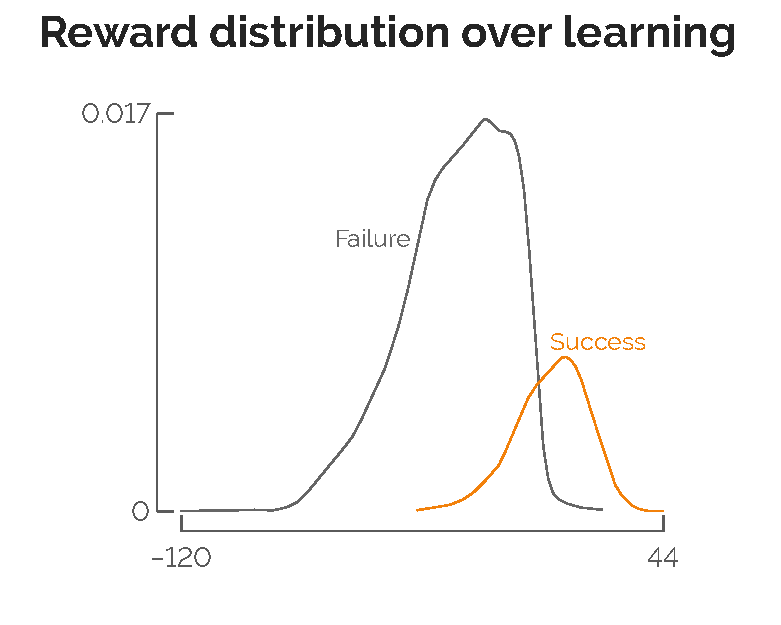
\includegraphics[width=0.49\textwidth]{Reward_status.pdf}
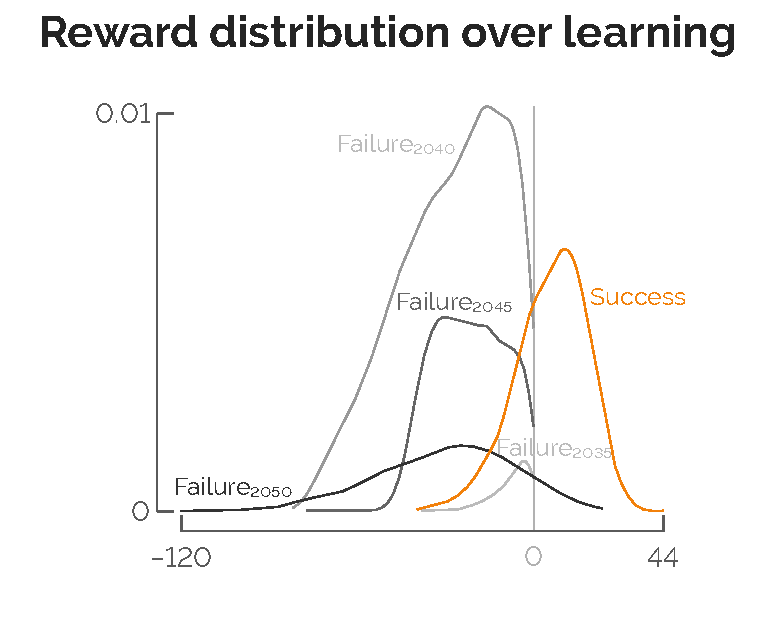
\includegraphics[width=0.49\textwidth]{Reward_status_2.pdf}
\caption{Reward distribution between successes and failures. Graph on the right hand side details at the end of which time-window the failure occurred. The ``tipping year'' is 2040 as failing the transition by 2040 represents 57\% of all the failures. Beyond this point, through this learning process, succeeding the transition represents 38\% of the episodes. }
\label{fig:reward_status}
\end{figure}

\newpage
Considering the end of the time-window where the \ce{CO2}-budget is exceeded, the right hand side of Figure \ref{fig:reward_status} shows that 2040 is the ``tipping year'' for the agent. Beyond this point, through this learning process, the chances to succeed the transition were 38\%. In other words, near-term (2025-2030) actions are necessary to hope succeeding the transition.

\subsection{States}
\label{subsec:RL:learning:states}

The first two dimensions of the state space are the cumulative emissions and costs. They drive the value of the reward and, consequently, the optimisation of the agent's policy. Per definition, the threshold of 1.2\,Gt$_{\ce{CO2},\text{eq}}$ splits the episodes reaching 2050 into successes and failures (see Figure \ref{fig:Cum_gwp_cost}). Since infeasible cases or those that overshoot the \ce{CO2}-budget are discarded before reaching 2050 (see Section \ref{subsec:RL:act_states_rew:rew}), the number of attempts that reach further steps in the transition progressively decreases. Consequently, the share of successful transitions compared to failures progressively increases with time. In the successful transitions, the median cumulative emissions, $\text{P}_{50}$, are about 0.9\,Gt$_{\ce{CO2},\text{eq}}$. Reaching cumulative emissions significantly lower than the \ce{CO2}-budget are possible thanks to efforts made at earlier stages of the transition and the potential to install \gls{SMR} later on. Considering the failures, half of these episodes ended up with cumulative emissions lower or equal to 1.4\,Gt$_{\ce{CO2},\text{eq}}$. As illustrated in Figure \ref{fig:reward_status}, 2040 is identified as the tipping year. Where 98\% of the failures were below the \ce{CO2}-budget in 2035, only 37\% passed this threshold in 2040. This reminds the importance of near-term, 2025-2030, actions to hope for a successful transition.

\begin{figure}[!htbp]
\centering
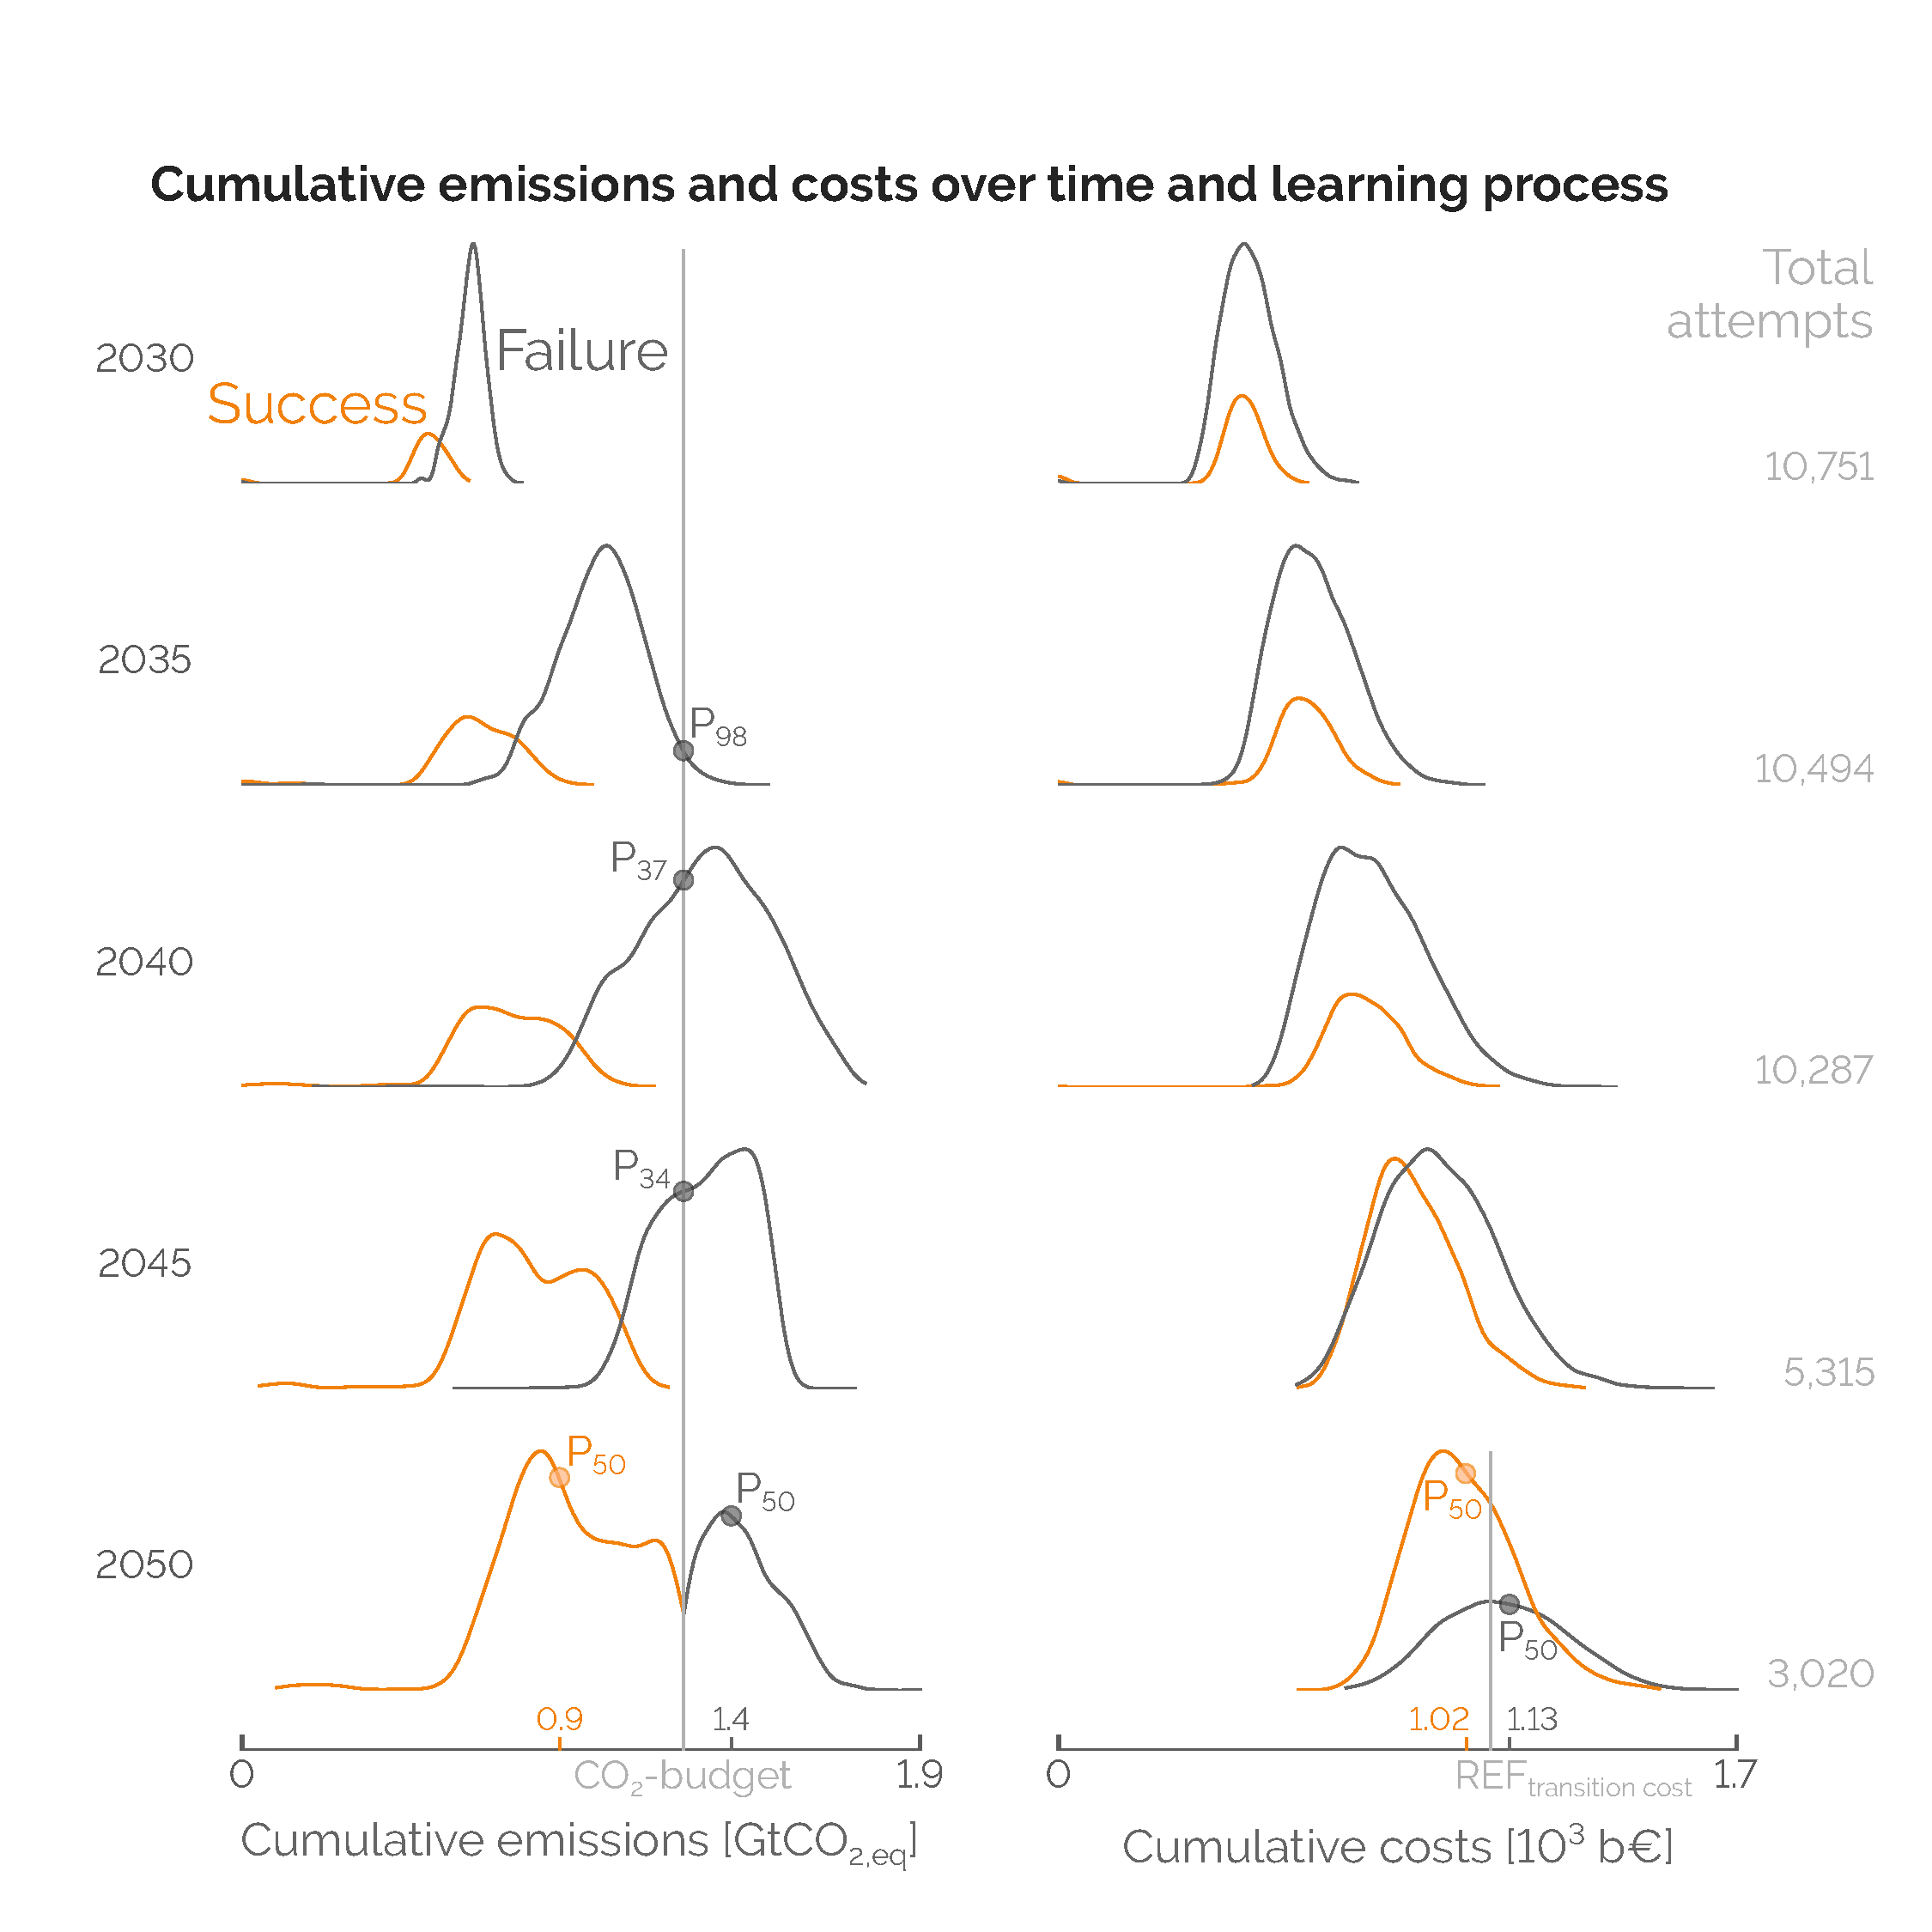
\includegraphics[width=0.8\textwidth]{Cum_gwp_cost_3.pdf}
\caption{Exploration of the state space over the learning process: distribution of occurrence of cumulative emissions (left) and costs (right). Number of remaining attempts decrease with time since infeasible problem and solutions overshooting the \ce{CO2}-budget are discarded prematurely, \ie before reaching 2050. Besides infeasible problems, distributions labelled as ``Failure'' represent the attempts that overshot the \ce{CO2}-budget by 2050 at the latest. The majority of successful transitions have cumulative emissions much lower than the \ce{CO2}-budget and are cheaper than the REF case. }
\label{fig:Cum_gwp_cost}
\end{figure}

\newpage
Given the reward function (see Figure \ref{fig:Reward}), the agent optimises its policy by aiming at lowering the total transition cost as soon as it meets the \ce{CO2}-budget. The skewness of the cumulative emissions and costs in 2050 are indications of this reward function (see Table \ref{tab:skewness_gwp_cost}). When succeeding the transitions, the cumulative emissions have a negative skewness: the agent successfully stayed within the budget and most of the cases where close to that budget (median at 0.9 Gt$_{\ce{CO2},\text{eq}}$). On the contrary, the cumulative cost of successful transitions has a positive skewness: the agent successfully reduces the cost of the system as a secondary objective with 30\% of the cases above the reference transition cost. This hierarchy of agent's objective is verified with the failures. When it failed the transition, the agent aimed at reducing the emissions (skewness of 0.61) before minimising the total transition cost (skewness of 0.24). 

\begin{table}[htbp!]
\caption{Skewness of cumulative emissions and costs in 2050. Cumulative emissions are skewed to the left and to the right for the successes and failures, respectively. The skewness of the cumulative costs for successful transitions is higher compared to failures. On top of being the results of the optimisation through EnergyScope, these are influenced by the agent's policy that aims only at lowering the total transition cost as soon as it meets the \ce{CO2}-budget.}
\label{tab:skewness_gwp_cost}
\centering
\begin{tabular}{l c c}
\toprule
\textbf{Status of episode}  & \textbf{Skewness of cumulative} & \textbf{Skewness of cumulative} \\
\textbf{in 2050}  & \textbf{emissions} & \textbf{costs} \\	
\midrule
Success & -0.52 & 0.50 \\
Failure & 0.61 & 0.24 \\
\bottomrule							

\end{tabular}
\end{table}

\newpage
Finally, we observe that the majority of the successful transitions are cheaper than the reference transition cost, 1.1\,b€. Among the parameters impacting the most the total transition cost, we observe that success occurs when, on average,  the cost of purchasing fossil fuels is increased more than the one of electrofuels (see Table \ref{tab:param_RL}). In other words, to have higher chances to succeed a myopic transition, the key factor is to reduce the uncertainty on the cost of purchasing electrofuels or to increase the cost of fossil fuels. Given the skewness that is positive and negative for the electrofuels and the fossil fuels, respectively, these cases represent more than the majority of the successful cases. On top of this, total transition costs of successful episodes are lower due to lower industrial \gls{EUD} and discount rate. These favourable conditions combined with the right agent's actions led to transitions respecting the \ce{CO2}-budget.

\begin{table}[htbp!]
\caption{Uncertain parameters impacting the most the total transition cost and, for the successful transitions, the mean of their values between 0 and 100\%, $\mu$, and their skewness, $\gamma$. On top of being supported by the agent's actions, successful transitions occur when the cost of purchasing fossil fuels is more increased than the one of electrofuels.}
\label{tab:param_RL}
\centering
\begin{tabular}{l c c c}
\toprule
\textbf{Parameter}  & \textbf{$\mu$} & \textbf{$\gamma$}  \\	
\midrule
Purchase electrofuels & 50.4\% & 0.004  \\
Industry EUD & 49.8\% & 0.026 \\
Discount rate & 48.4\% & 0.089\\
Purchase fossil fuels  & 55.0\% & -0.068\\
\bottomrule							

\end{tabular}
\end{table}

Besides the cumulative emissions and costs, the agent also observes the share of renewable energy carriers in the primary mix and the efficiency of the system The share of renewable energy carriers in the primary mix allows identifying intermediate milestones along successful transitions (see Figure \ref{fig:RE_in_mix_Efficiency}). From the initial state of 10\% in 2020, a boost of integration of renewables in the near-term is needed to hope for a successful transition. For the successful occurrences to exceed failures, this share increases to 54\% in 2025. Along the transitions, this increase goes with the import of electrofuels and the full deployment of local \gls{VRES}. In 2050, the threshold where occurences of success are more numerous than failures was at 82\% of renewable share. In the REF case of Chapter \ref{chap:atom_mol}, this share reached 86\% by 2050. However, by 2050, Figure \ref{fig:RE_in_mix_Efficiency} shows another ``bump'' at lower share of renewables in the mix. This area corresponds to the possibility to install \gls{SMR}. As uranium is considered as a non-renewable resource \cite{rixhon2021terminology}, installing \gls{SMR} allows lowering the threshold as in the SMR case of Chapter \ref{chap:atom_mol}. Besides these milestones to respect the \ce{CO2}-budget of the transition, one can also look at the other side of the thresholds. Below the near-term threshold of $\sim$60\%, this is the ``no-go zone'' where succeeding the transition becomes unlikely, except if betting on the future installation of \gls{SMR}.

The efficiency, as defined in Section \ref{sec:RL:act_states_rew}, gives less valuable information towards successful transitions. Through the transition, besides the share of success increasing over the failures, the distributions of success and failure indistinguishably spread over the whole range. Similarly than the emissions, we observe a bump at lower efficiencies by 2050 due to the installation of \gls{SMR}.

\begin{figure}[!htbp]
\centering
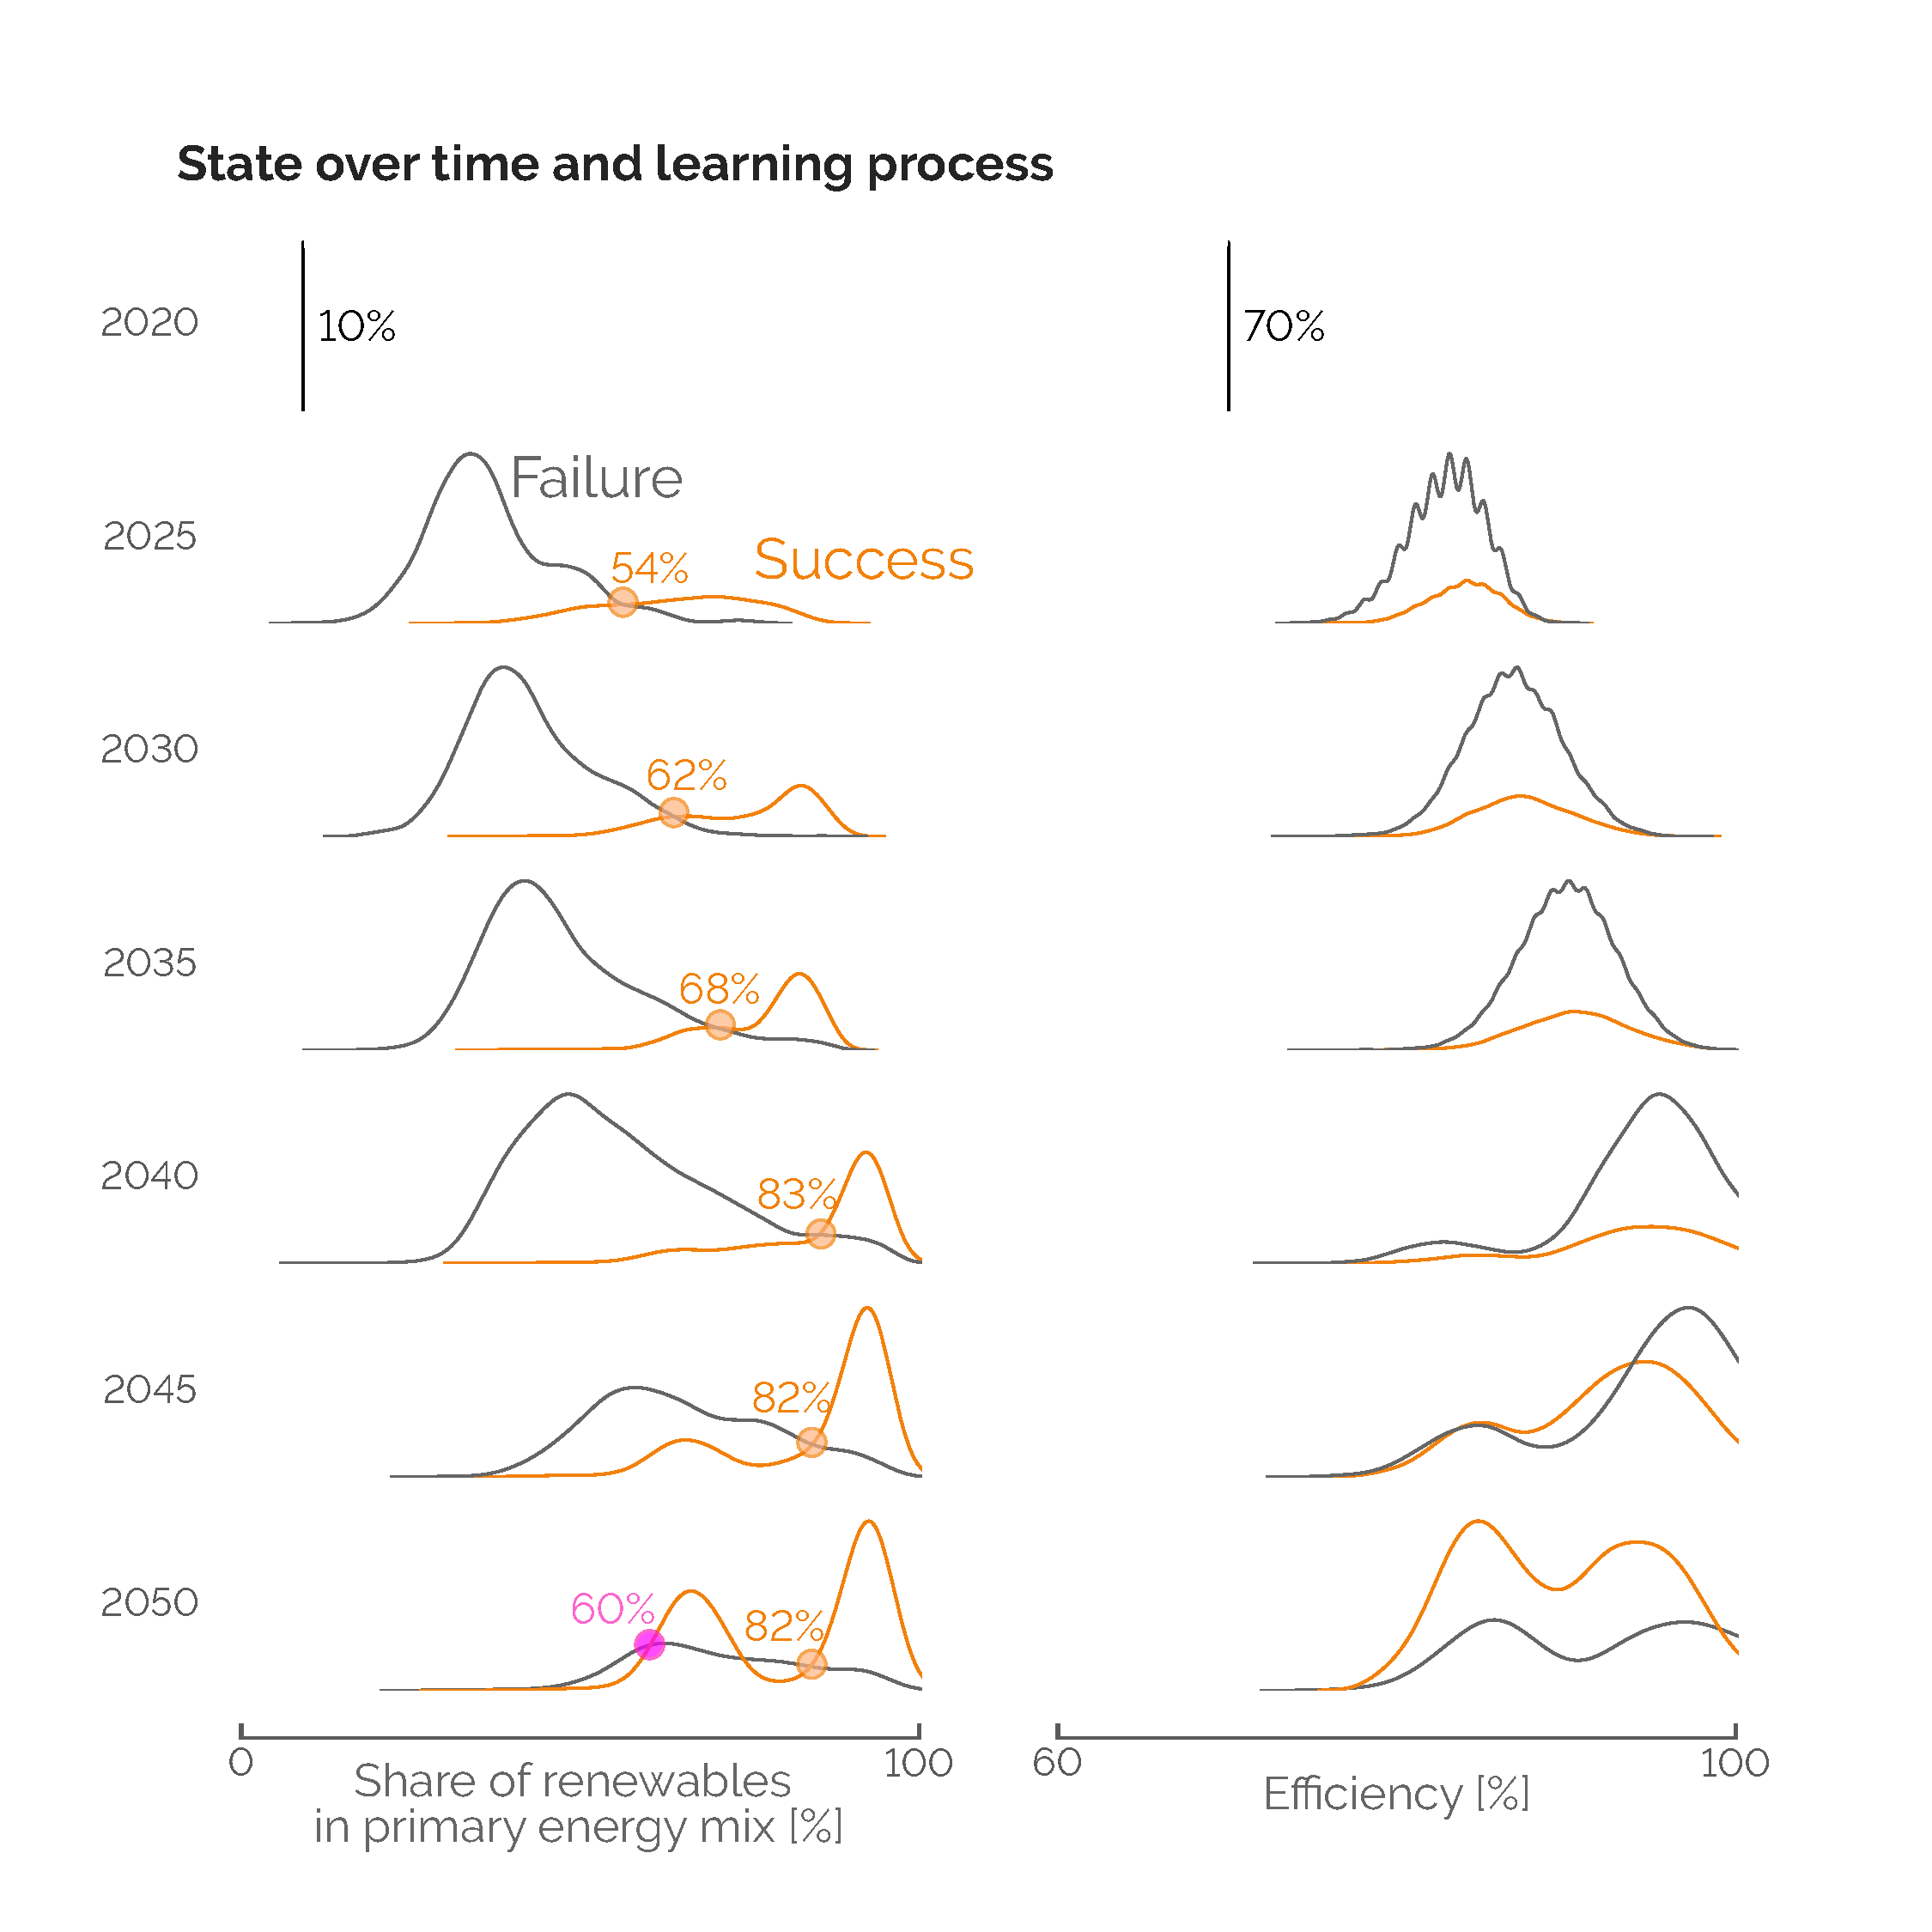
\includegraphics[width=0.8\textwidth]{RE_in_mix_Efficiency.pdf}
\caption{Exploration of the state space over the learning process: distribution of occurrence of share of renewable energy carriers in the primary energy mix (left) and efficiency (right).  Number of remaining attempts decrease with time since infeasible problem and solutions overshooting the \ce{CO2}-budget are discarded prematurely, \ie before reaching 2050. Besides infeasible problems, distributions labelled as ``Failure'' represent the attempts that overshot the \ce{CO2}-budget by 2050 at the latest. Integration of local \gls{VRES} at early stages then massive import of electrofuels later are needed to secure successful transitions. Below a near-term threshold ($\sim$60\%), the chances of success are limited, \ie no-go zones. Efficiency is a less valuable information for the agent to succeed transitions as failures and successes indistinguishably spread over the whole range.}
\label{fig:RE_in_mix_Efficiency}
\end{figure}

\subsection{Actions}
\label{subsec:RL:learning:actions}

After investigating the intermediate milestones to meet the \ce{CO2}-budget by 2050, this section details the actions the agent has taken during the learning process (see Figure \ref{fig:Actions_learning}). Rows represent the beginning of the time window at which the set of actions is taken. Similarly to the state space, we observe a wide exploration of the action space. The more the agent was able to progress through transition, without exceeding the \ce{CO2}-budget, the bigger is the share of successes compared to failures. Besides this observation, no specific range of values for the different actions at the different timing seems to lead to more successes. Looking at action individually, there does not seem to be any that supports more effectively the transition. The success come from the combination of these actions.

\begin{figure}[!htbp]
\centering
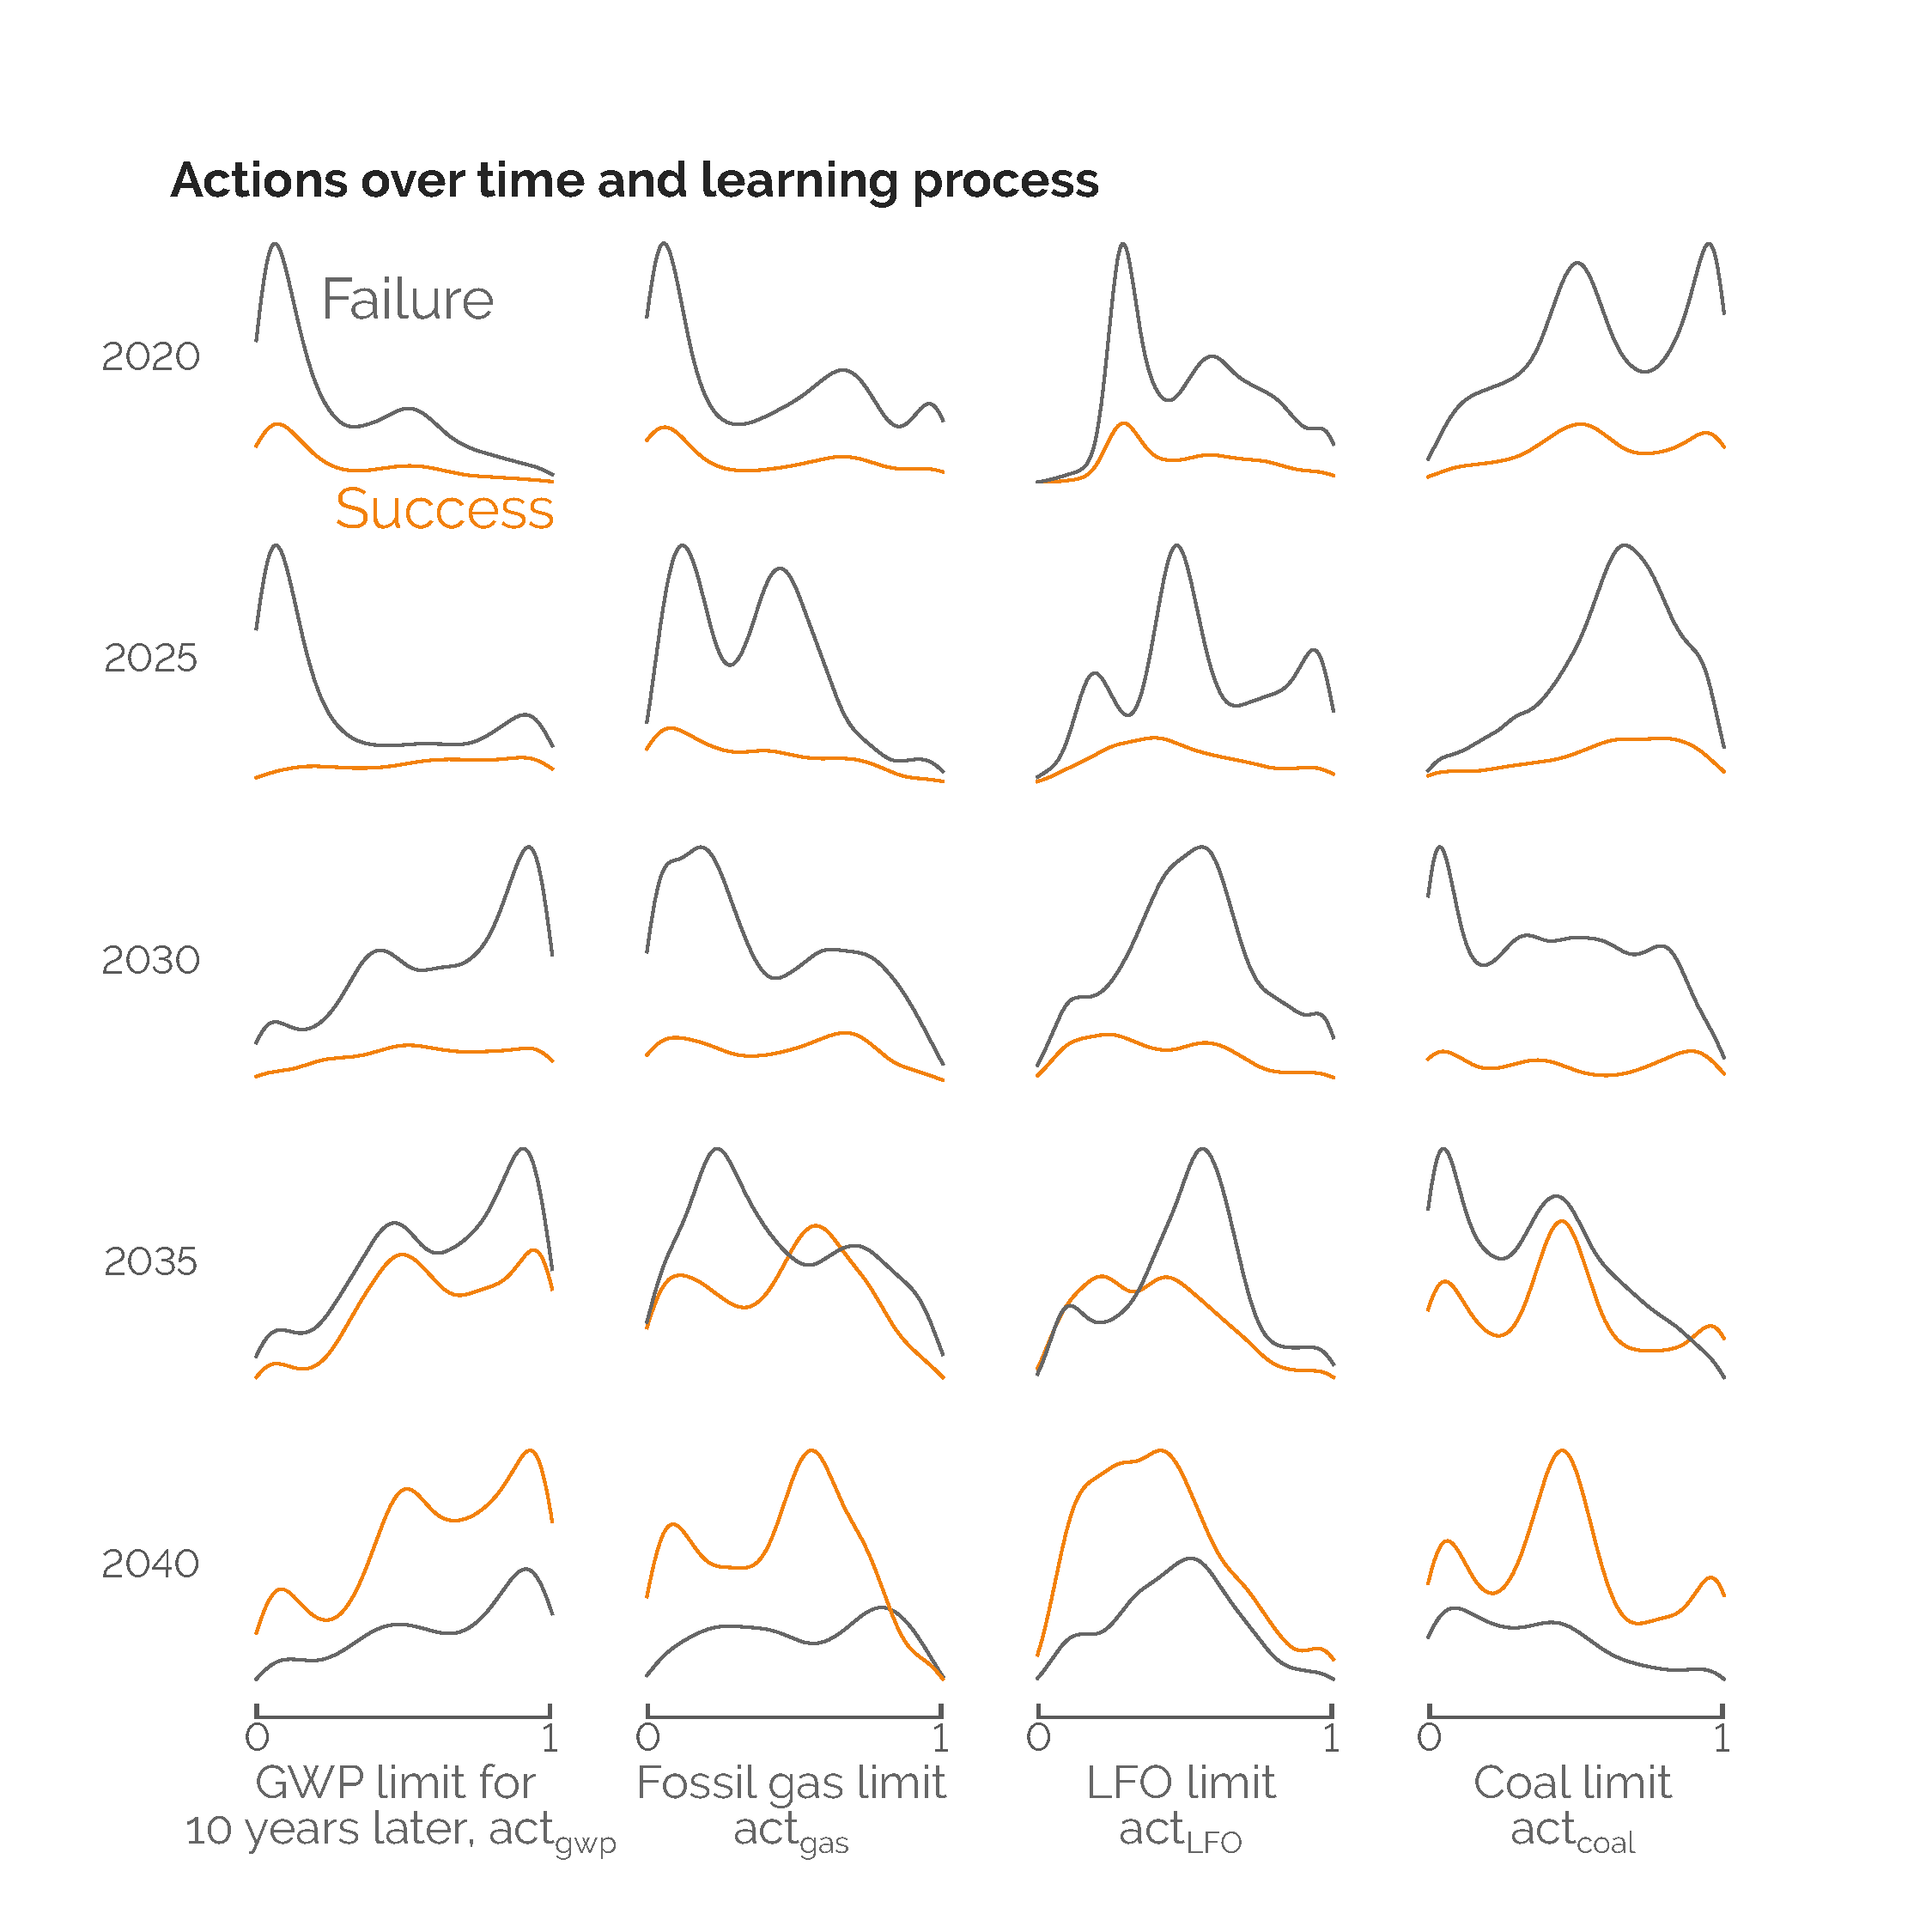
\includegraphics[width=0.8\textwidth]{Actions_learning.pdf}
\caption{Exploration of the action space over the learning process: distribution of occurrence of the different actions at the time they are taken by the agent. Number of remaining attempts decrease with time since infeasible problem and solutions overshooting the \ce{CO2}-budget are discarded prematurely, \ie before reaching 2050. Besides infeasible problems, distributions labelled as ``Failure'' represent the attempts that overshot the \ce{CO2}-budget by 2050 at the latest. Besides this wide exploration, successes and failures indistinguishably spread over the whole ranges of actions. In other words, it does not seem to be any clear set of actions to support successful transitions.}
\label{fig:Actions_learning}
\end{figure}

To identify the actions that have an actual impact on the environment, we can check if they are binding or not. In a \gls{LP} problem, constraints represent hyperplanes in the domain of variables. In a two-dimension space, these are straight lines (see Figure \ref{fig:Binding_constr}). When the problem is bounded and feasible, these lines are the edges of a convex polygon: the domain of feasibility. The optimal solution, $\textbf{x}^*$, is the combination of variables leading to the optimal value of the objective function. Besides being within the domain of feasibility, it is proven that this optimal solution, when unique\footnote{There are cases where the objective function has the same optimal value along an entire edge. In this case, there is an infinity of solutions and the problem is indeterminate.}, locates on a vertex of the domain \cite{bertsimas1997introduction}. The constraints intersecting at this vertex are considered as binding, actually limiting the objective function to be more optimal. In other words, binding constraints, when tightened, aggravate the objective value function. If these are inequality constraints, as represented in Figure \ref{fig:Binding_constr}, it means that their left and right sides of the equation are equal.

\begin{figure}[!htbp]
\centering
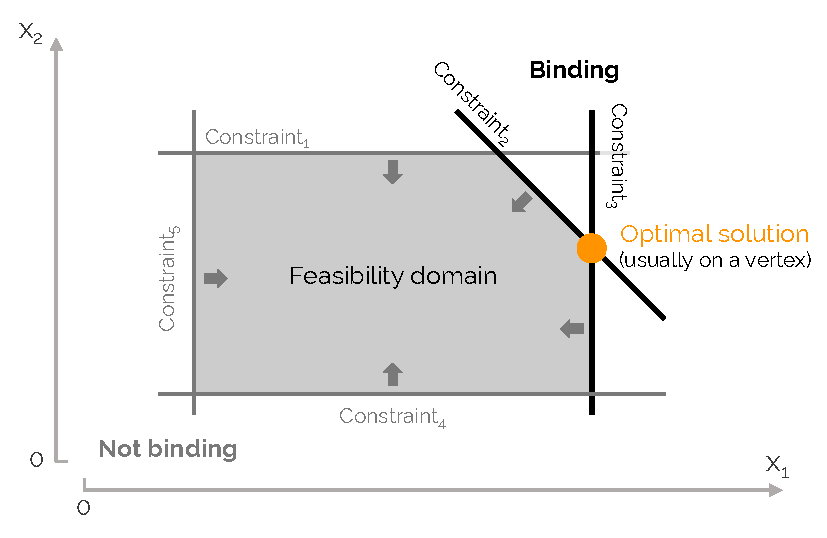
\includegraphics[width=0.7\textwidth]{Binding_constr.pdf}
\caption{Binding versus non-binding constraints. In \gls{LP} where the feasibility domain is non-empty and bounded, the constraints defined a convex feasibility domain in the space of variables (here, x$_1$ and x$_2$). The optimal solution usually locates on a vertex of this domain, \ie the intersection of several constraints (here, constraints 2 and 3) limiting the solution. These constraints are considered as binding, \ie having a limiting impact on the optimal solution.}
\label{fig:Binding_constr}
\end{figure} 

After filtering out failures of the learning episodes and keeping only the successful transitions, only a limited set of the actions are binding and have an actual impact on the result of the optimisation in EnergyScope Pathway (see Figure \ref{fig:Binding_learning}). This allows identifying key actions to support the myopic transition. Limiting the \gls{GWP} in the near-term is a key-factor for success. However, this action has a binding effect on the environment only at the end of the transition. The range over which limiting the use of fossil gas binds the optimisation is wider. Compared to other non-renewable fuels, this is due to the longer use of this energy carrier favoured by its low \gls{GWP} (the second after uranium) and its versatility (applications in the electricity, heat and mobility sectors). In line with \citet{vogt2018starting}, the early constraints on generation and the sharper decrease of the emissions avoid lock-in situations.

\begin{figure}[!htbp]
\centering
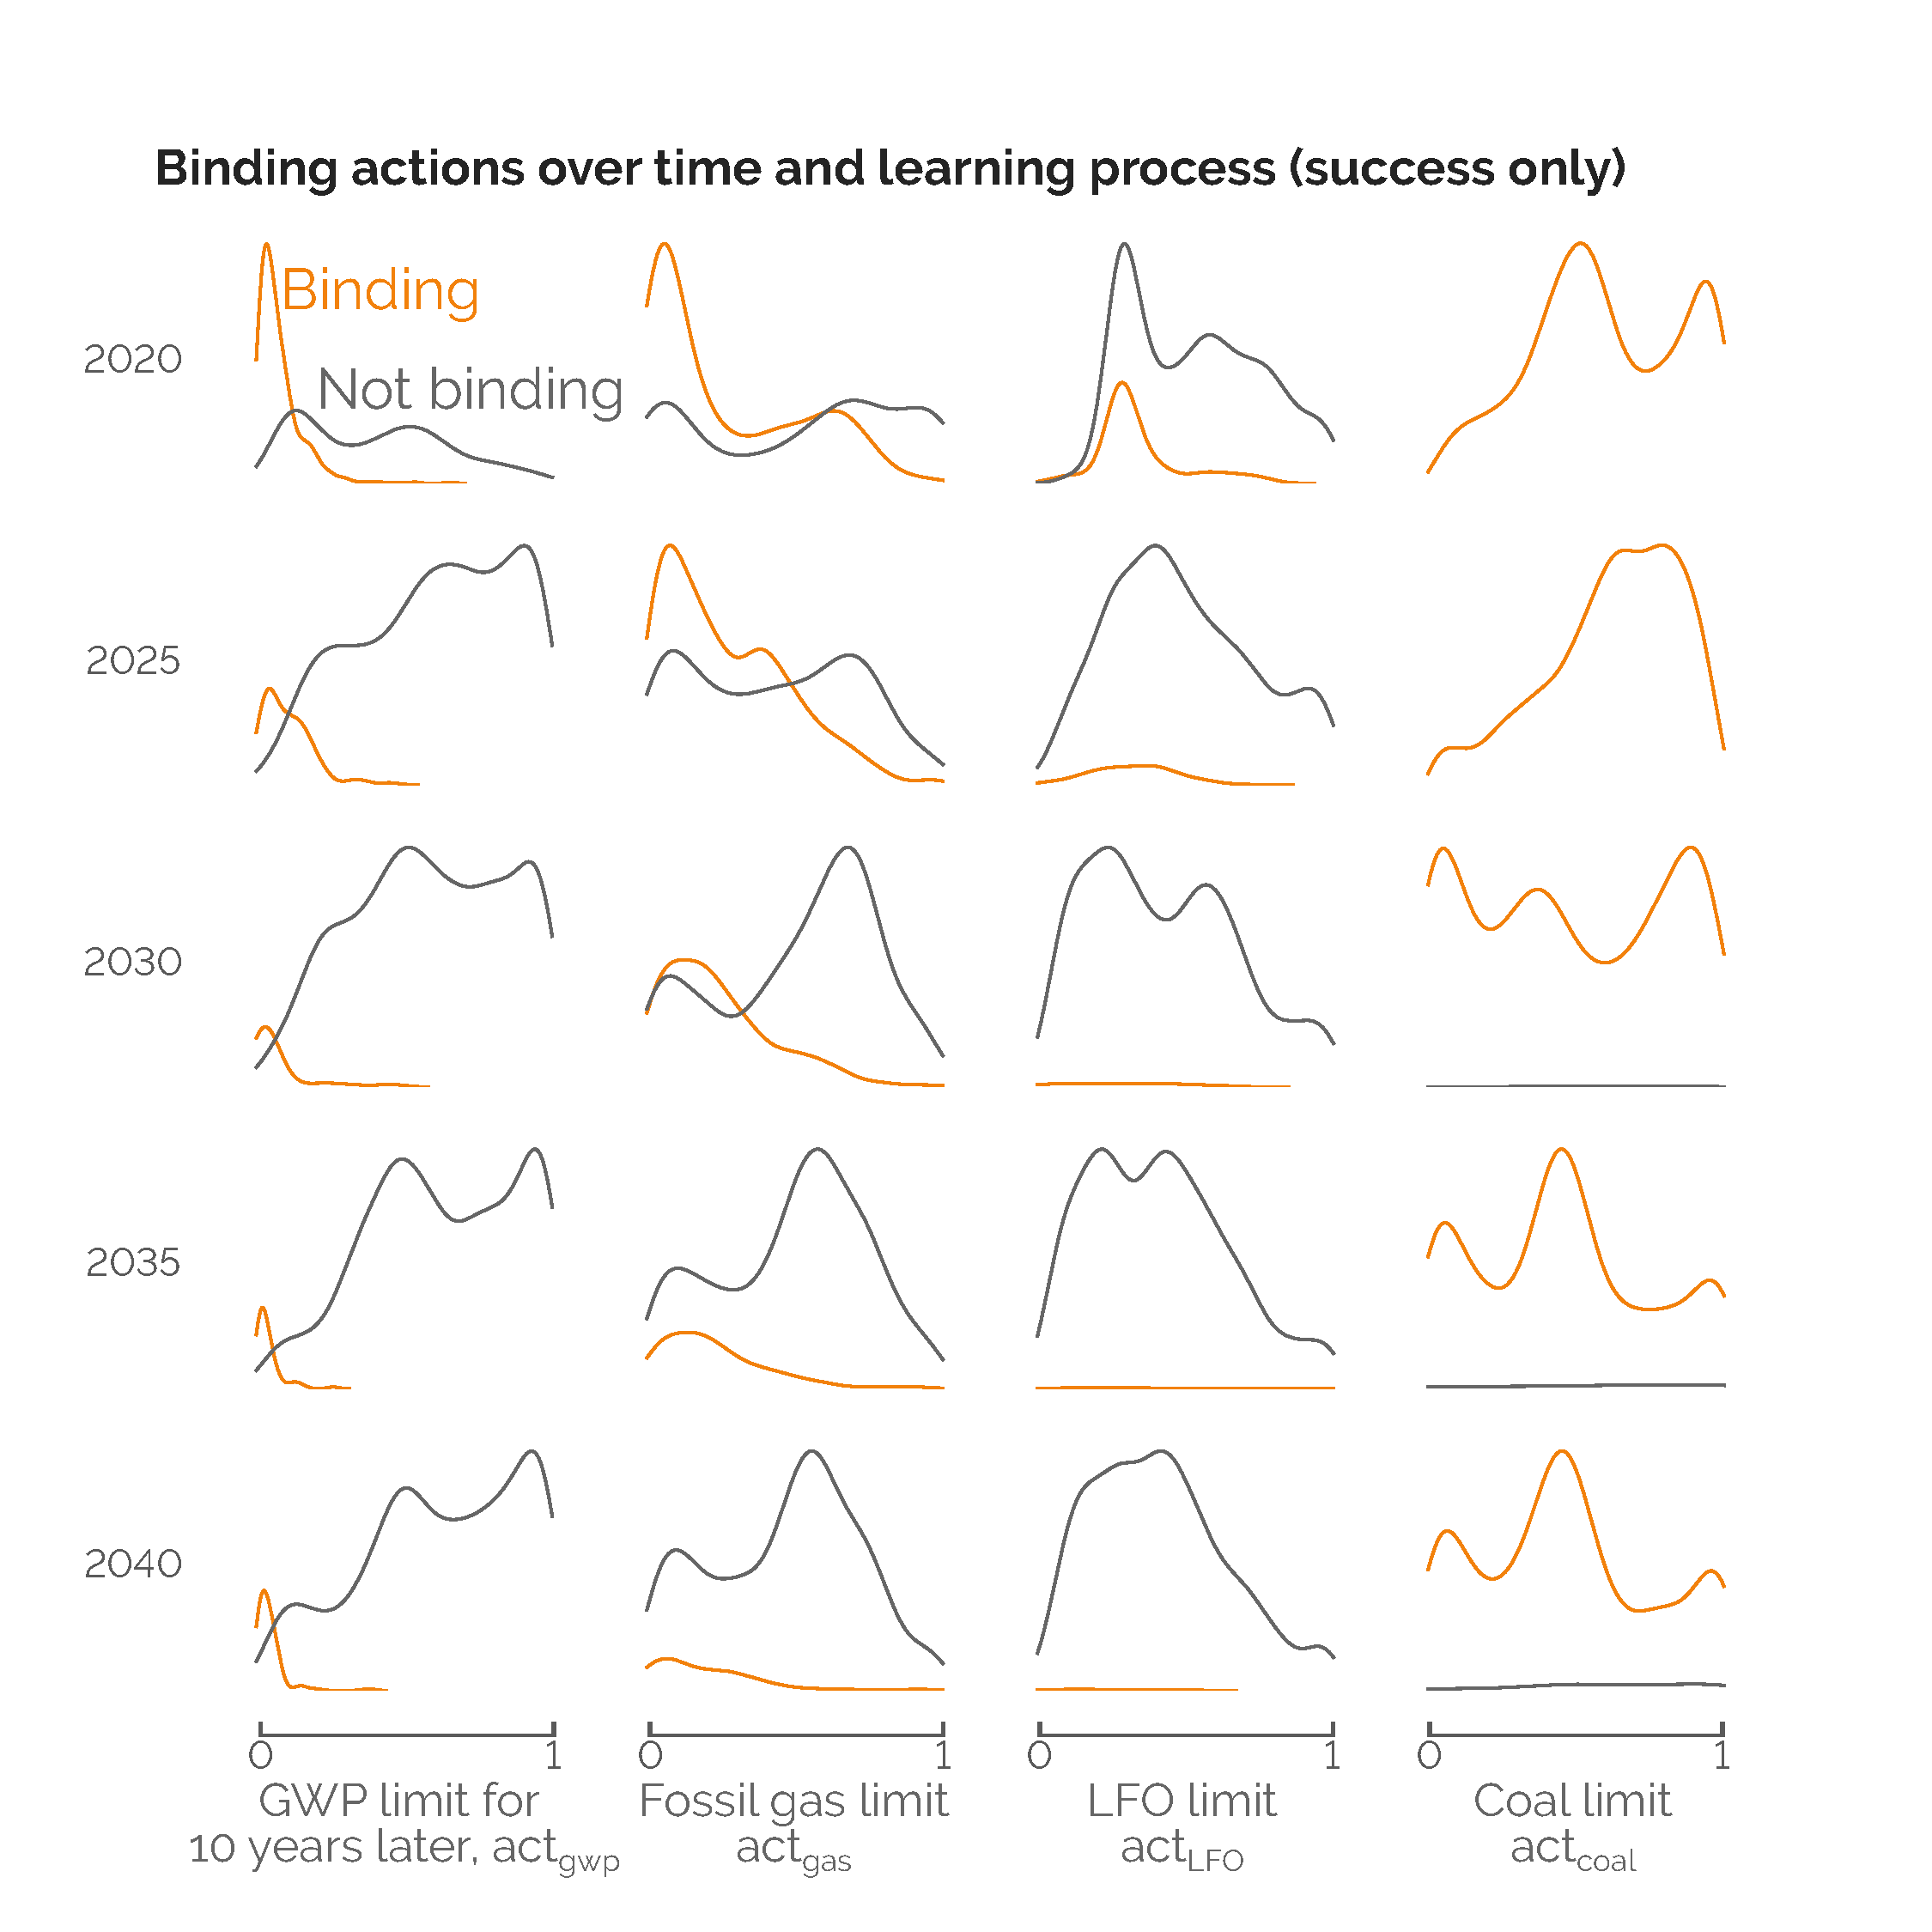
\includegraphics[width=0.8\textwidth]{Binding_learning.pdf}
\caption{Keeping only the successful transitions, distribution of occurrence of binding and not binding actions. Depending on the action and its timing, it is actually constraining the optimisation through EnergyScope Pathway or not. Sweet spots can be identified when considering the limits of \gls{GWP} and fossil gas consumption. Limiting coal consumption is always constraining, unlike \gls{LFO} that is ``naturally'' substituted by EnergyScope Pathway in the near-term.}
\label{fig:Binding_learning}
\end{figure}

When it comes to limiting the use of \gls{LFO} and coal, the conclusions are more straightforward. At the beginning of the transition, most of the 159\,TWh of \gls{LFO} are consumed by naphtha-cracker (46\%) and decentralised boilers (45\%). The remaining 10\% are consumed by industrial boilers. Even though \gls{LFO} represents  30\% of the primary energy mix in 2020, the cost-optimum removes it of the mix without requiring the action of the agent. Naphtha-crackers, decentralised and industrial boilers get substituted by \gls{MTO}, decentralised \gls{HP} and industrial resistors and \gls{CHP}, respectively.  This ``non-bindness'' of limiting \gls{LFO} is an indication that this action could be removed from the agent's levers of action without impacting the optimisation of its policy.

On the contrary, limiting coal is always binding. Before all, this is due because coal is a cheap resource (17\,€/MWh). In other words, the cost-driven environment will favour it. Then, as the maximum amount of coal (28\,TWh) is much smaller than fossil gas and \gls{LFO}, high value of $\mathrm{act}\textsubscript{coal}$ still represents small consumption of coal.

\subsection{Discussion and guidelines for future researchers}
\label{subsec:RL:act_states_rew:discussion}
As introduced in Chapter \ref{chap:chap_methodo}, most of the work in applying \gls{RL} is the definition of the interactions between the agent and its environment (\ie actions, reward and states) that are very dependent on the case study and the research questions to answer. The elements presented in this work result from several trial and errors to end up with meaningful results according to our research questions.

Besides mimicking potential actual policies, the actions chosen in this work have a direct translation into constraints and we can therefore assess their effectiveness through the fact they are binding or not. In this work, we have investigated other actions like incentivising solar \gls{PV} panels and wind turbines by ``artificially'' reducing their \gls{CAPEX}. The result was not conclusive as these technologies need to take part to the Belgian energy transition and because it was harder to assess the impact of this action. 

The reward function was designed to first aiming at respecting the \ce{CO2}-budget then minimising the total transition cost. The -300 penalty given in case of an infeasible optimisation problem was arbitrarily set. \textit{A posteriori}, it seems to be a well-defined penalty given its significant relative difference with the values taken by the reward otherwise, between -120 and 44 (see Figure \ref{fig:reward_status}). Besides this penalty and given the observed results, we recommend to start with the same reward function if the objective is similar, first target cumulative emissions then cumulative costs. This requires to define the \ce{CO2}-budget according to a certain sharing principle (see Section \ref{sec:cs:CO2-budget}) and to compute reference total transition cost. However, other researches focusing on reaching carbon-neutrality by 2050 could define a binary reward function as +1 for reaching the objective and -1 otherwise.

Finally, states aim at representing the information relevant to the agent to efficiently learn and progress through the transitions. For this reason, on top reward-related features (cumulative emissions and costs), we added other indicators that are actually monitored to help decision-makers assessing their policies to reach their targets (share of renewables in the mix and the system overall efficiency). For other studies, one might consider other information like the metrics considered by \citet{pickering2022diversity} (\eg heat electrification, average national import or level of curtailment).

In conclusion, future studies might start from the actions-reward-states defined in this work and adapt these rules depending on the research questions to answer, the case study and the energy system optimisation model.

\newpage
\section{Comparison with references}
\label{sec:RL:testing}
After investigating the exploration of myopic transition, this section compares these results with the perfect foresight under uncertainties from the \gls{UQ} analysis presented in Chapter \ref{chap:atom_mol}. To reduce the computational time, the monthly model could also be used to carry out \gls{RL}-based exploration of myopic pathways. Appendix \ref{app:app_RL_TD_MO} presents the comparison between the results obtained from the learning process on the hourly and monthly models.

\gls{RL}-based myopic optimisation provides \ce{CO2}-emissions pathways different from the perfect foresight approach to respect the same \ce{CO2}-budget (see left side of Figure \ref{fig:Gwp_pathway_total_tran_cost}). However, driven first by this \ce{CO2}-budget, the agent often reaches much lower cumulative emissions when succeeding the transition (see Figure \ref{fig:Cum_gwp_cost}). This comes from the agent's actions that limit the emissions and/or the consumption of fossil resources at the early stages. Thanks to the bigger reduction of emissions at these early stages, the \gls{RL}-based optimisation can benefit from a ``\ce{CO2}-buffer'' at the end of the transition. This buffer is compensated by the end of the transition where 50\% of the myopic transitions reach 2050 with 10 or more remaining Mt$_{\ce{CO2},\text{eq}}$ compared to 4 for the perfect foresight approach. These remaining emissions by 2050 come from the consumption in industrial boilers of waste and coal that account for 3.5\% and 2.4\% on average by 2050. Finally, the long-term vision of the perfect foresight approach results in smoother reduction of the emissions to end up with less emissions by 2050.

The comparison between the failures and the pathways demonstrates the added-value brought by myopic pathway optimisation. In the near-term (2025-2030), levels of emission are similar between perfect foresight and myopic cases that have failed. This shows that limited foresight encourages to strongly act at the early stages. On top of this, following the initial steps of \ce{CO2}-emissions pathways resulting from PF approach would likely ($\sim$80\%) lead to fail the transition. 

Looking at the total transition cost, the combination of the agent's actions and favourable economic conditions (see Section \ref{subsec:RL:learning:states}) make the myopic transitions cheaper, on average, than the PF cases (see right side of Figure \ref{fig:Gwp_pathway_total_tran_cost}). This is also due to the fact that the perfect foresight approach always finds a solution even in worst conditions such as high cost of purchasing resources and high \gls{EUD}. This explains the wider variability of the results too. However, with the same sample of uncertain parameters, given the assumed full knowledge over the whole time horizon, PF naturally results in a cheaper transition than its myopic equivalent.

\begin{figure}[!htbp]
\centering
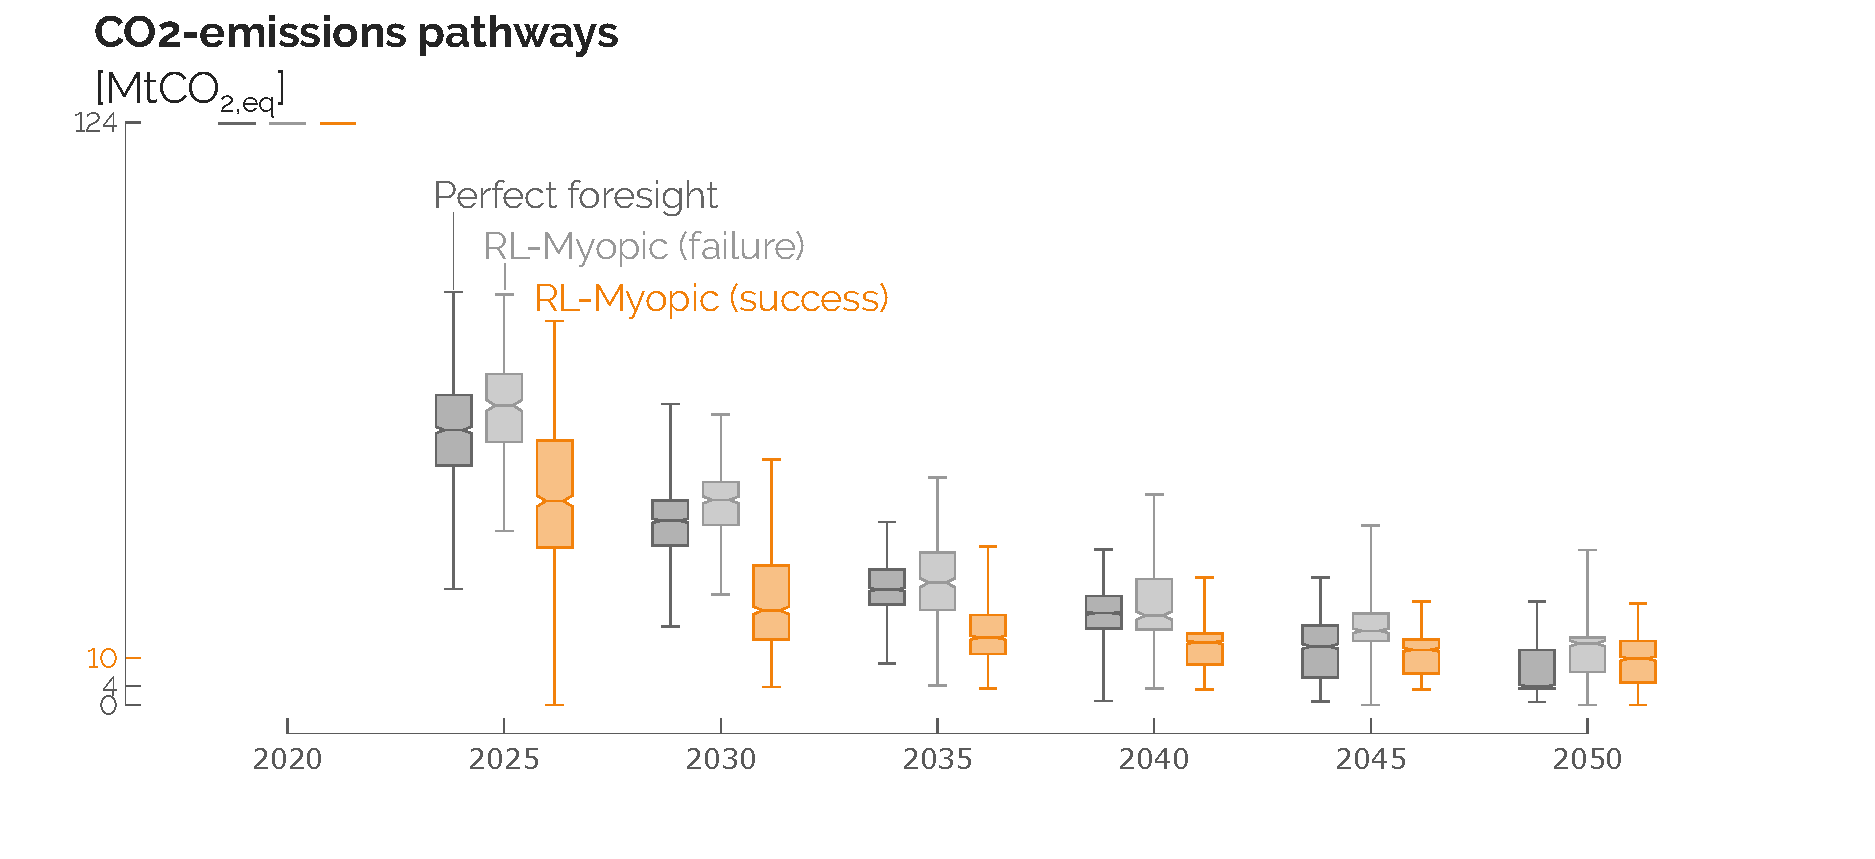
\includegraphics[height=3.5cm]{Gwp_pathway_core.pdf}
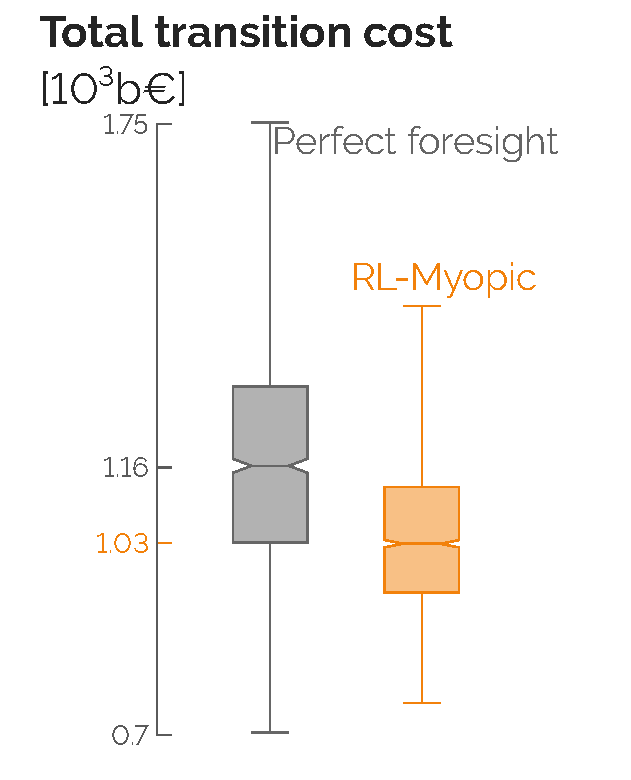
\includegraphics[height=3.5cm]{Transition_cost_comp_2.pdf}
\caption{Comparison of \ce{CO2}-emissions pathways (left) and total transition cost (right) from the perfect foresight optimisation under uncertainties and the \gls{RL}-based myopic optimisation. Myopic transitions succeed with a more drastic reduction of emissions in the short-term and, on average, more favourable economic conditions.}
\label{fig:Gwp_pathway_total_tran_cost}
\end{figure}

%The transition pathways of the annual system cost show another impact of the agent in the \gls{RL}-based exploration (see Figure \ref{fig:System_cost_pathway}). Via its actions and its cost-based reward, the agent can reach systems that are cheaper than any other solution obtained by the perfect foresight approach. The perfect foresight approach gives a wider variability in its cost since this method always found a solution even in worst conditions such as high cost of purchasing resources and high \gls{EUD}. 

%\begin{figure}[!htbp]
%\centering
%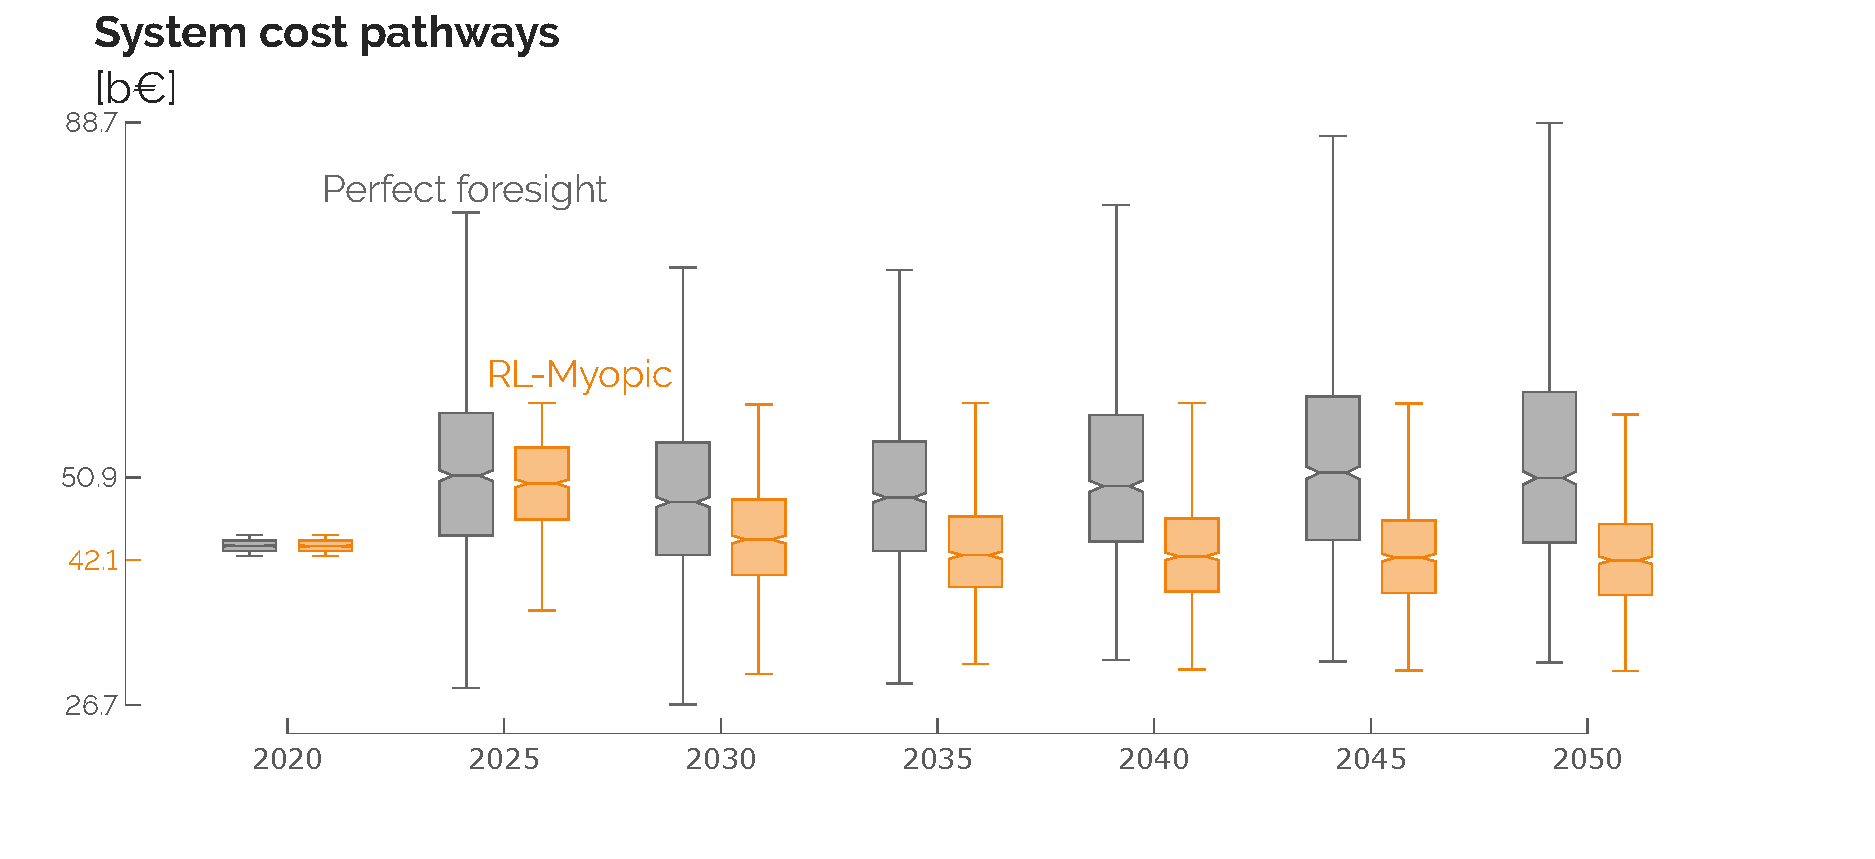
\includegraphics[width=0.8\textwidth]{System_cost_pathway_core.pdf}
%\caption{Comparison of annual system costs pathways from the perfect foresight optimisation under uncertainties and the \gls{RL}-based myopic optimisation.}
%\label{fig:System_cost_pathway}
%\end{figure}

\newpage
The analysis of the cumulative costs shows that the \gls{OPEX} is the main difference between myopic and perfect foresight transitions (see Figure \ref{fig:Opex_Capex_Salvage_comp}). Supported by the agent's actions, successful myopic transitions have a lower \gls{OPEX} than the perfect foresight ones.

\begin{figure}[!htbp]
\centering
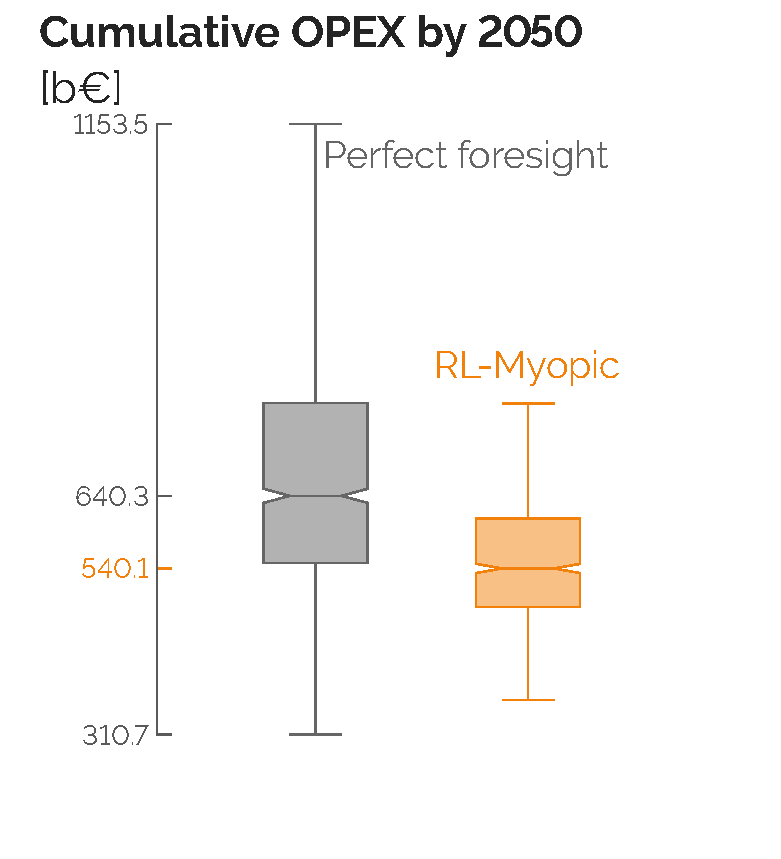
\includegraphics[width=0.325\textwidth]{Opex_2050_comp_core.pdf}
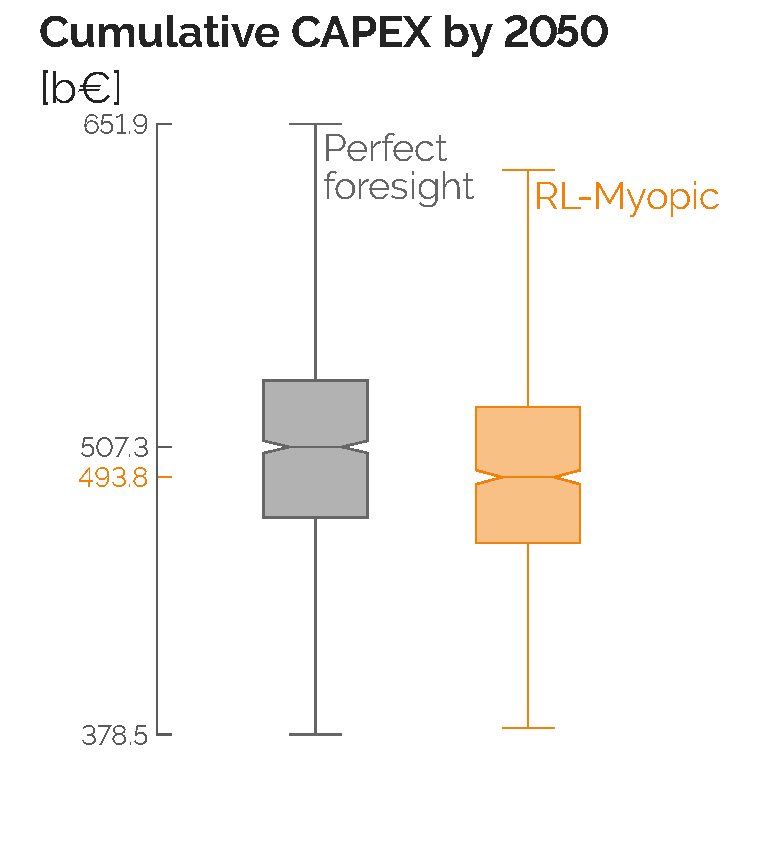
\includegraphics[width=0.325\textwidth]{Capex_2050_comp_core.pdf}
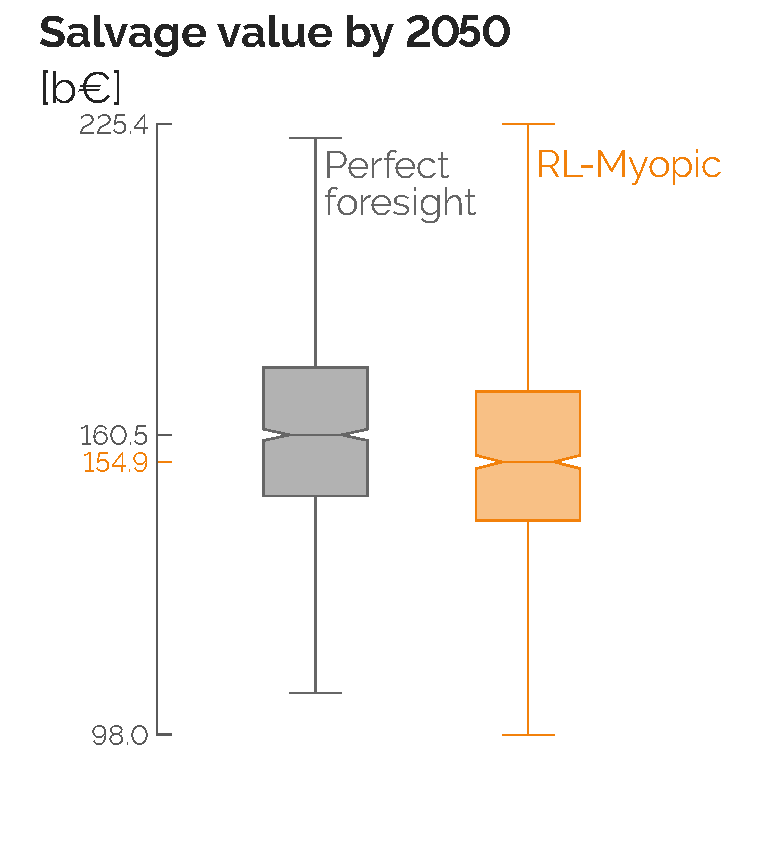
\includegraphics[width=0.325\textwidth]{Salvage_2050_comp_core.pdf}
\caption{Comparison of cumulative OPEX (left), CAPEX (center) and salvage value (right) in 2050 from the perfect foresight optimisation under uncertainties and the \gls{RL}-based myopic optimisation.}
\label{fig:Opex_Capex_Salvage_comp}
\end{figure}

The cost of purchasing the energy carriers represents about 70\% of the total cumulative \gls{OPEX}. The assessment of the primary energy mix by 2050 highlights that the difference of OPEX between the perfect foresight and the myopic pathways come from the import of electrofuels, and especially of e-ammonia (see Figure \ref{fig:Mix_2050_comp}).  In the majority of the cases, e-ammonia is more than two times more imported in the myopic transitions. Being cheaper than e-methane (see Chapter \ref{chap:case_study}), e-ammonia brings flexibility in the production of electricity via \gls{CCGT} (see Chapter \ref{chap:atom_mol}). Besides the slightly favourable economical conditions (see Table \ref{tab:param_RL}), the myopic optimisations opt to invest massively into importing renewable molecules because of the limited knowledge in the future, and, among others, the availability of \gls{SMR}. This explains why 50\% of the successful transitions reached cumulative emissions below 900\,Mt$_{\ce{CO2},\text{eq}}$ (see Figure \ref{fig:Cum_gwp_cost}).

\begin{figure}[!htbp]
\centering
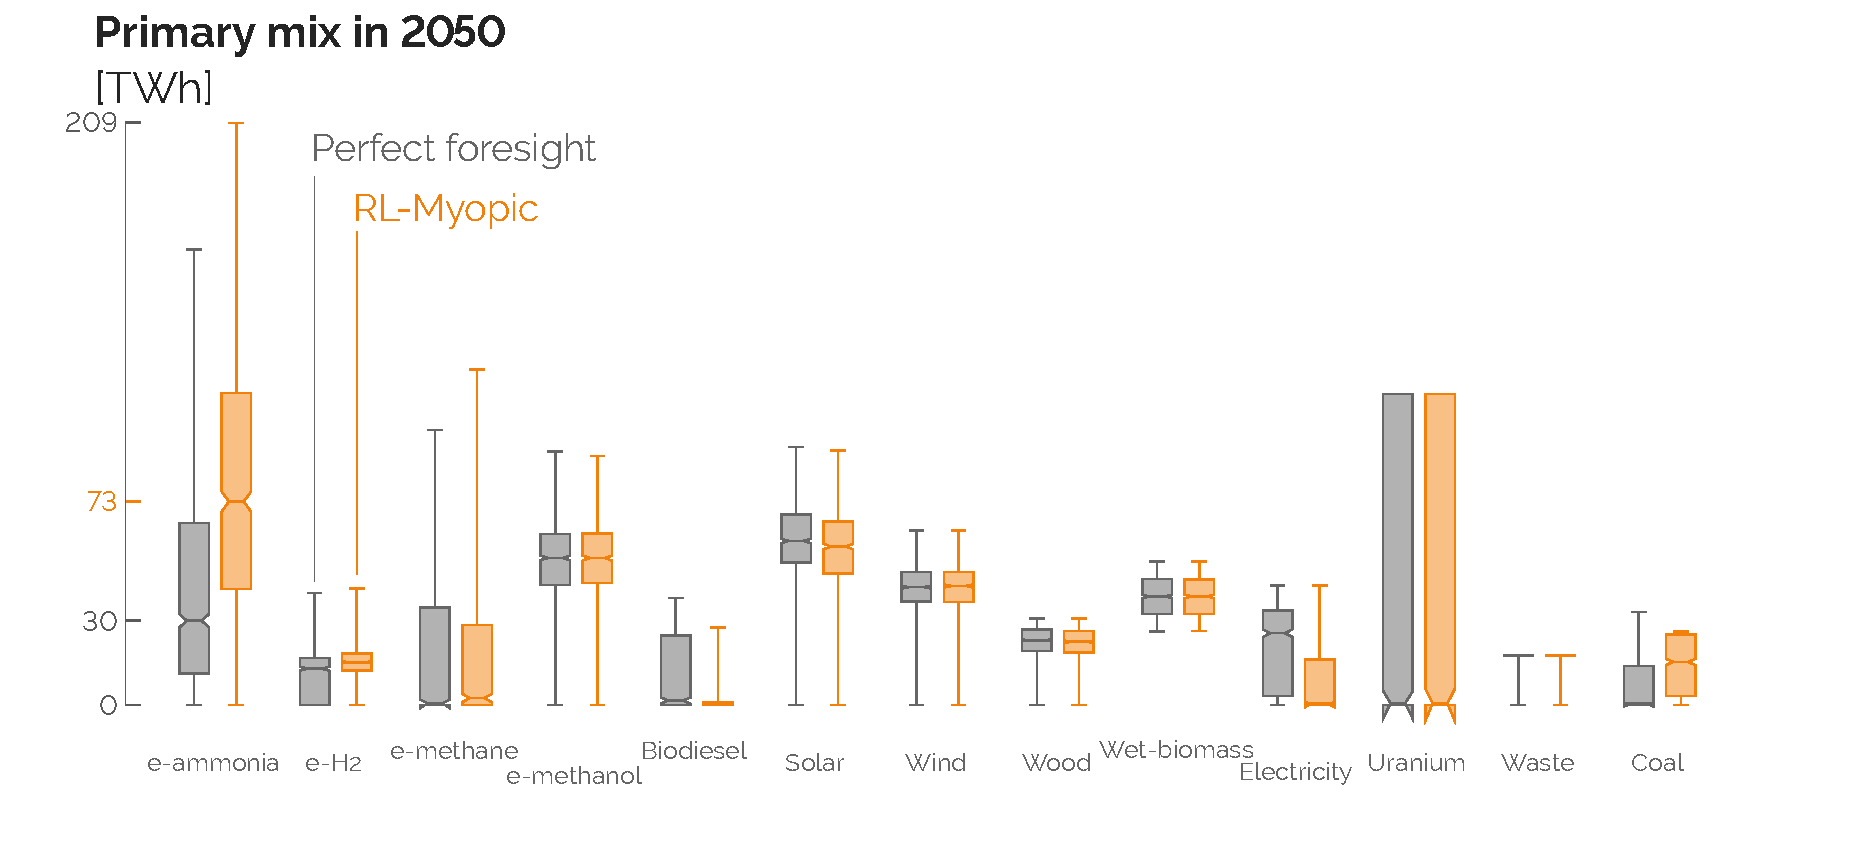
\includegraphics[width=0.8\textwidth]{Mix_2050_comp_core.pdf}
\caption{Comparison of the primary energy mix in 2050 from the perfect foresight optimisation under uncertainties and the \gls{RL}-based myopic optimisation. The biggest difference is about e-ammonia to supply \gls{CCGT}.}
\label{fig:Mix_2050_comp}
\end{figure}


\section{Conclusions}
\label{sec:RL:conclusions}
In the literature, two options are investigated to explore transition pathways of a whole-energy system: perfect foresight and myopic. In perfect foresight optimisation, a full knowledge of the parameters is assumed over the entire time horizon. To add more realism, myopic optimisation considers a sequence of more limited time windows leading to the end of the time horizon \cite{poncelet2016myopic}. To respect a \ce{CO2}-budget over the transition, this case requires a prescribed \ce{CO2}-trajectory \cite{fais2016impact}. However, since the effect of \ce{CO2}-emissions in climate change is cumulative, the total amount of these emissions matters more than the trajectory itself. Consequently, we have applied the \acrfull{RL} approach on the environment of the Belgian myopic pathway optimisation under uncertainties.

%In the \gls{RL} framework, the agent had four actions to support the 2020-2050 transition: (i) limiting the \ce{CO2}-emissions at the end of each successive time window and limiting the consumption of (ii) fossil gas, (iii) \acrfull{LFO} and (iv) coal. The reward fed back by the environment to the agent focused first on meeting the \ce{CO2}-budget, 1.2\,Gt$_{\ce{CO2},\text{eq}}$ equivalent to 10 years at the current level of emissions. A secondary focus is also put on aiming at a minimum transition cost. To know its progress through the transition, the agent has the information of the cumulative emissions and costs as well the share of renewable energy carriers in the primary energy mix and the system overall efficiency.

This \gls{RL}-based exploration pointed out that short-term actions were needed to hope succeeding such a transition, as also demonstrated by \citet{luderer2018residual}. Where \gls{LFO} becomes less cost-competitive in the near-future, limiting the use of coal should be done at any cost. Then, fossil gas should be replaced by e-methane in the mid-term while putting a strict limit on the overall emissions becomes the most effective action by the end of the transition. The analysis of the share of renewables in the primary energy mix highlighted intermediate milestones to have higher chances to succeed the transition. Below 54\% of renewables in the mix in the near-future, these chances become much more limited, \ie the no-go zone. 

We have compared the results coming from this \gls{RL}-based myopic optimisation with the hourly perfect foresight approach. These myopic optimisations provided pathways respecting the \ce{CO2}-budget that were more drastic in cutting emissions in the short-term than the perfect. Supported by the agent's actions, we could reach cheaper energy system than what the perfect foresight could give. This comparative analysis also pointed out that investing more into renewable electrofuels was the option when knowledge about the future is limited. To do so, it requires reducing the uncertainties of their cost of purchasing. 

Further analyses should assess more accurately the impact of uncertainties on the agent's capacity to succeed the myopic transition. These analyses would aim at identifying the parameters that should necessarily be in specific ranges to allow the agent to succeed. On the contrary, there could be ranges of values for which the chances of success would be much more limited.

In conclusion, via the application of the \gls{RL} approach, we have widely explored the different myopic transition pathways and identified sweet-spots (and no-go zones) to succeed a transition with an ambitious \ce{CO2}-budget target. It also highlighted the actions to take to effectively support a whole-energy system transition.